\chapter{Microclimate study of plant in wind tunnel}
\label{ch:microclimatestudy}
\def\figdir{chapters/ch05_microclimatestudy/figures/}

\textit{This chapter is based on the paper under preparation Manickathan et al., 2019}.

\section{Introduction}

\lettrine[lines=3,nindent=0em,loversize=0.1]{T}{he} influence of plants on the microclimate in an urban environment is a growing interest due to the need of suppressing detrimental effects of urbanization and climate change \citep{Chen2006,Demuzere2014,Dimoudi2003,Matthews2017,Shashua-Bar2009b,Shashua-Bar2000}. Plants modify the climate by intercepting solar radiation, extracting heat from the environment during photosynthesis \citep{nobel2009physicochemical}. Furthermore, the plant element interferes with the airflow extracting the momentum and enhance turbulent mixing \citep{Finnigan2009, Gromke2014, Sanz2003}. Due to the present growing need to ensure cities are resilient and can mitigate the adverse effects of climate change, there exists a need to ensure accurate prediction of the influence of mitigation strategies such as vegetation. Several numerical approaches are employed to study the impact of vegetation \citep{Alexandri2008,Gromke2011,Manickathan2018a,Yang2017}. However, these models reduced the plant complexity by simplified parameterization, that is typically derived from various plant response measurements. Thus, there is a great need for high-resolution, accurate measurement for the development of such numerical models and their subit sequent validation.

Various experimental approaches ranging from field measurements, greenhouse measurements and wind tunnel measurement have been used to study the response of plants. The benefit of field measurement is that can provide an in-situ understanding on the performance of the plants in an urban environment \citep{Grant1998,Koizumi2016,Shashua-Bar2009b,Shashua-Bar2000}. Whereas, studies in greenhouses can provide better control on the environmental conditions but focuses on smaller potted plant species \citep{Fatnassi2006,Ganguly2009,Majdoubi2009,Montero2001}. Such studies also complement numerical simulations and cross-comparison \citep{Boulard2002, Kichah2012, Majdoubi2009}. However, the greatest control on the wind flow condition is obtained in wind tunnel experiments \citep{Grace1977, Liu2018, Manickathan2018b,Miri2019}.

Furthermore, it to accurately parameterize the influence of the vegetation, the plant geometry and its porosity distribution have to be known. Typical techniques to determine the leaf area density (LAD) distribution of the plant is through optical techniques consisting of imaging the sides of the plant \citep{Cao2012, Grant1998, Guan2003, Manickathan2018b, Phattaralerphong2005} or by destructive techniques requiring the defoliation of the plant \citep{Jonckheere2004, ONeal2002}. From these approaches, the leaf area distribution is approximated, and porosity is estimated. However, such approaches either provide a simplified estimation of the plant porosity, uncertainty in the spatial variability or are destructive technique, causing a detrimental impact on the plant and disable it from further experiments thereafter. However, x-ray computed tomography (x-ray CT) approach can be a mean to estimate the plant morphology, and it is a typical technique to estimate the porosity of various build materials \citep{Lal2017,Parada2017,Patera2018} and pipelining with additional experiments. Some studies have shown the feasibility of the technique to perform non-intrusive data acquisition of plant element characteristics \citep{Brodersen2013, Dhondt2010}.

Therefore, wind tunnel experiments provide a level of control over the inflow conditions that is seldom possible with greenhouse and infeasible in an in-situ measurement campaign. However, such studies typically focus on the aerodynamic aspects of plant and only very few on the climate responses of the plant \citep{Grace1977}. Furthermore, a combined detailed study on the plant morphology is seldom performed. The influence of plant morphological variability such as the plant porosity is known to have a significant impact on the flow conditions \citep{Bitog2011,Cao2012,Manickathan2018b}. Moreover, simultaneous measurement of spatiotemporal variability of the leaf temperature to the diurnal cycle has not be performed to the authors’ knowledge. The feasibility of employing infrared thermography to obtain leaf temperature variability has been demonstrated in the past \citep{Jones1999,Merlot2002}.

Thus, in the present study, we investigate the influence of plant morphology and its spatial variability on the microclimatic. The diurnal response of the plant is evaluated to determine additional temporal variability. Furthermore, the influence of various environmental condition such as wind speed and solar radiation intensity on the plant performance is studied. The goal of the present study is to obtain a holistic understanding of plant performance, where the plant morphology is its derived plant traits such as leaf area, leaf area, leaf area density, and plant porosity are measured using x-ray computed tomography (x-ray CT), the plant wake turbulence is measured using particle-image velocimetry (PIV), various climate conditions such as air temperature and relative humidity are measured using climate sensors and leaf temperature distribution is measured using infrared thermography. The combined measurement is performed for a single isolated plant (Buxus sempervirens) inside a wind tunnel, providing a high-resolution dataset for future validation studies. Thus, the present study aims at answering the following questions: What are the spatial and temporal variability of the plant performance due to environmental conditions such as wind speed and solar radiation? What is the diurnal response of the plant? 

\section{Materials and Methods}

\subsection{Materials}

The multi-measurement campaign for a detailed plant morphology measurement and the resulting climatic response is performed for a small Buxus plant (\textit{Buxus sempervirens}) as shown in \cref{fig:plant_setup}. The plant foliage is having a bounding box of $20\times20\times21$ cm$^3$ ($x\times y \times z$, i.e., streamwise, spanwise and vertical) as shown in \cref{fig:plant_setup}b. The plant resides in a sealed pot to ensure water loss is only through leaf transpiration \cref{fig:plant_setup}c. The plant pot is sealed using the kneadable putty sealant. The water loss due to transpiration is periodically compensated by $1$\% (vol.) fertilized water (NPK 7-4-6 buxus fertilizer). The pre-experiment setup consists of periodically irrigation and exposing to artificial sunlight with a 12-hour day-night cycle consisting of fixed-intensity 12-hour photoperiod. The plant acclimation to the upcoming experimental condition is performed for around $1$ week. The artificial sunlight is provided using an Osram Ultra-Vitalux $300$ W solar simulator bulb, generating $13.6$ W of UVA and $3.0$ W of UVB. The bulb is placed $60$ cm above the plant canopy to provide $100$ W~m$^{-2}$ plant-canopy incident short-wave radiation. Furthermore, the growth of the plant foliage is periodically maintained to ensure the desired plant geometry as shown in \cref{fig:plant_setup}. The detailed measurement of the plant morphology including geometry, porosity distribution, leaf size distribution and total leaf area is obtained using the high-resolution x-ray tomography measurement.

\begin{figure}[t]
	\centering
	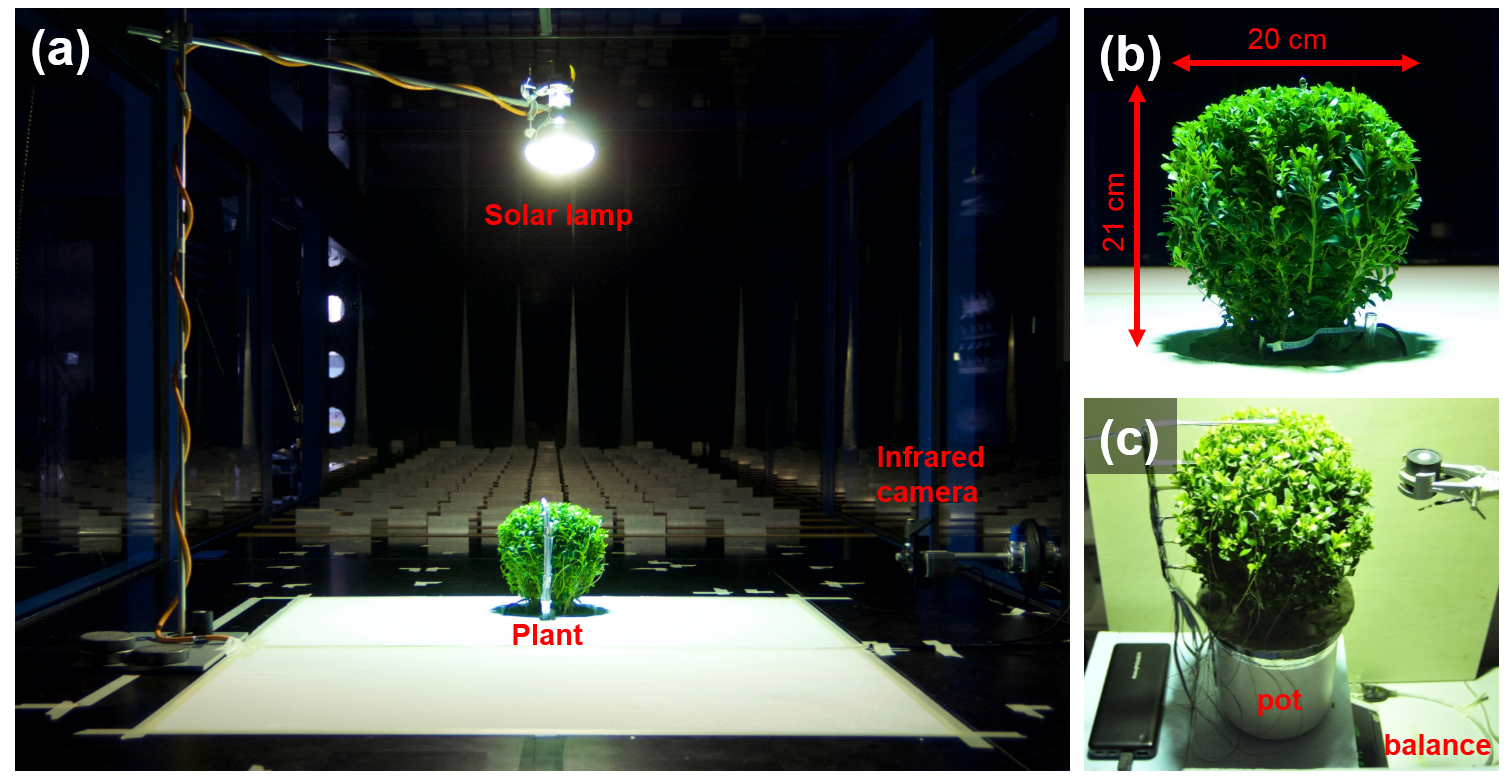
\includegraphics[width=\textwidth]{\figdir/plant_setup.png}
	\caption{Wind tunnel setup for combined microclimate, PIV and infrared thermography measurements: \subfig{a} Microclimate measurement setup as illustrated in \textbf{Fig. 4b}, \subfig{b} A close-up frontal-view (windward) of the plant foliage, \subfig{c} pre-experiment plant acclimation setup.}
	\label{fig:plant_setup}
\end{figure}


\subsection{Experimental setup and procedure}

The experimental campaign is divided into three stages: pre-experimental controlled acclimation setup, plant morphology ``\textit{offline}'' measurement and wind tunnel ``\textit{online}'' experiment. The pre-experiment control setup is where the plant is maintained providing the necessary cyclic artificial sunlight and nutrition. Furthermore, the sensors required for measuring in-plant air and leaf temperature and air humidity is mounted at this stage. The second stage is the \textit{online} experiment inside the wind tunnel where the flow field downstream of the plant, microclimate inside the plant, net transpiration rate and the plant foliage thermal profiles are measured. The equilibrium condition and the dynamic response of the plant for a given radiation and wind intensity are measured. The final stage of the campaign consists of measuring the plant morphology and is performed using a high-resolution x-ray imaging \cref{subsec:xray}.

\subsection{X-ray imaging}
\label{subsec:xray}
An x-ray imaging technique is used to obtain the high-resolution computation tomography (X-ray CT) dataset of the plant. Various plant properties such as foliage morphology, plant porosity distribution and the net leaf area can be derived from the scan. The advantage of such an approach is that it is a non-intrusive approach and can, therefore, be pipelined into a series of additional experiments \citep{Lal2017,Patera2018}. The plant specimen measurement is performed at the Diagnostic Imaging Clinic, Vetsuisse Faculty, University of Zurich (``\textit{Tierspital}''), under the supervision of Dr. Richter. The x-ray imaging is performed with Philips Brilliance CT 16-slice scanner, shown in \cref{fig:xrayimaging}, designed for medical imaging with an acquisition period of $39$ seconds. The CT slices have a resolution of $0.318\times0.318$  mm$^2$ pixel with a slice thickness of $0.4$ mm. The 12-bit image intensity data and the associated metadata of the measurement are stored in conjunction inside the DICOM file format. Finally, a 3D voxel distribution of X-ray attenuation of the biological sample, represented in Hounsfield units, is obtained. The plant properties such as net leaf area are obtained from the 3D dataset after image processing, consisting of image enhancement, image segmentation, and classification (\cref{subsec:xraytomo}). 

\begin{figure}[t]
	\centering
	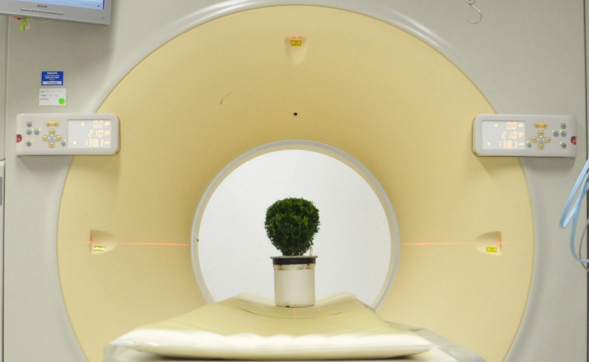
\includegraphics[width=0.7\textwidth]{\figdir/xrayimaging.png}
	\caption{X-ray imaging setup of the plant specimen at Diagnostic Imaging Clinic, UZH (``\textit{Tierspital}'') under the supervision of Dr. Richter. The specimen is imaged with Philips Brilliance CT 16-slice scanner, a medical imaging device.}
	\label{fig:xrayimaging}
\end{figure}


\subsection{Wind tunnel setup}
\label{subsec:windtunnelsetup}

The “online” measurement consists of microclimate measurement, where humidity, temperature, and net transpiration rate are measured and airflow measurement, where the wake-flow of the plant is measured. The measured are performed inside the ETHZ / Empa Atmospheric Boundary Layer (ABL) wind tunnel, a closed circuit Göttingen type wind tunnel with a test section cross-section of $1.9\times1.3$ m$^2$ ($W\times H$). The blockage ratio resulted from the plant is $1.7$\%. \cref{fig:plant_setup}a shows the wind tunnel setup that is employed to ensure minimal disturbances from measurement instruments. During the microclimate measurement, the diurnal variation of the air temperature and humidity distribution are recorded using thermocouples and RH/T sensors. Furthermore, the leaf temperatures are measured using an infrared thermography. Additionally, the net transpiration rate from the plant is measured using a mass balance hidden below the wind tunnel through an access panel, ensuring that the disturbance of the air flow is minimized  (\textbf{Fig. 4b}). The coupled measurement setup can be considered as a holistic measurement approach for simultaneously measuring multiple microclimate parameters. Thereafter, the airflow behind the plant is measured using particle image velocimetry (PIV).
	
	\begin{figure}[p]
		\centering
		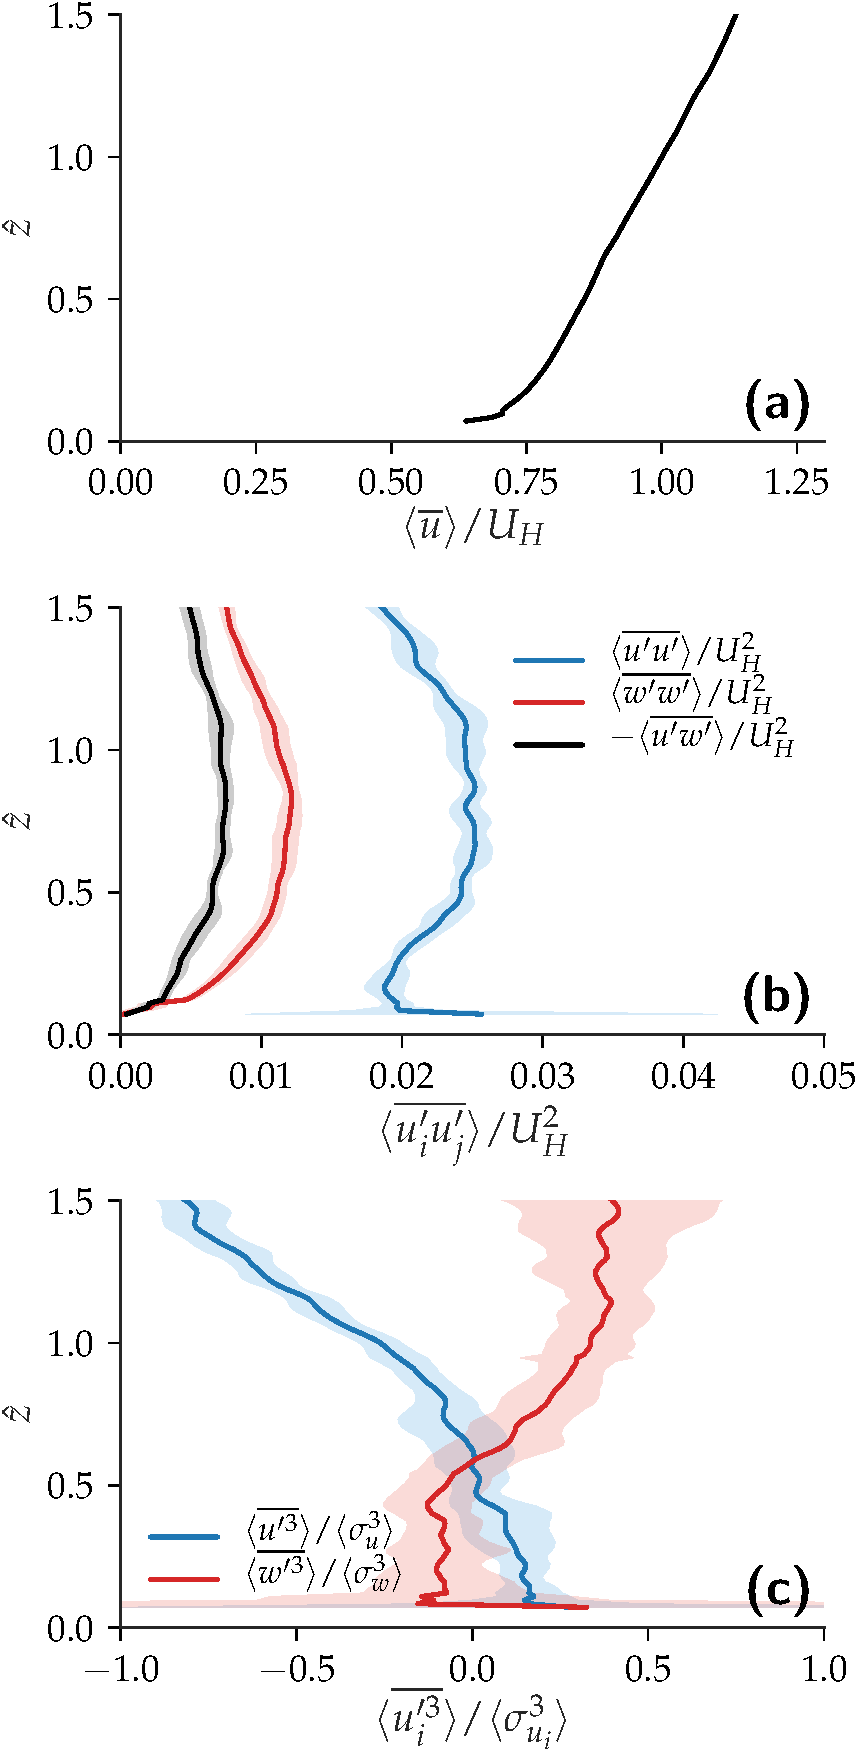
\includegraphics[height=0.9\textheight]{\figdir/figure_incomingvelocityprofile-crop.pdf}
		\caption{Vertical profiles of incoming \subfig{a} normalized mean streamwise velocity $\langle \overline{u} \rangle / U_H$, \subfig{b} normalized Reynolds stresses $\langle \overline{u'_i u'_j}/U_H^2 \rangle$ and \subfig{c} normalized skewness of streamwise $\langle \overline{u'^3} \rangle / \langle \sigma_{u}^3 \rangle$ and vertical velocity $\langle \overline{w'^3} \rangle / \langle \sigma_{w}^3 \rangle$. The canopy velocity at $H=210$ mm is $U_H = 0.77$ m~s$^{-1}$.}
		\label{fig:incomingvelocityprofile}
	\end{figure}

\subsubsection*{Microclimate boundary conditions}
A parametric study on the steady-state and dynamic response of the plant to multiple environmental conditions is performed: two wind tunnel set wind speeds, $0$ and $1$ m~s$^{-2}$, and two plant-canopy incident solar radiation, $0$ and $100$ W~m$^{-1}$. The air temperature and the relative humidity inside the wind tunnel is $21$ $^{\circ}$C and $25$\% RH, where the condition regulated by the HVAC system of the wind tunnel facility, triggered only after a large variation. However, in our study, as the input thermal energy from the wind tunnel system for the maximum wind speed ($1$ m~s$^{-1}$) and with the presently used solar lamp is low, the equilibrium temperature is seen not to deviate noticeably. 

\cref{fig:incomingvelocityprofile} shows the vertical profiles of the mean streamwise velocity and the Reynolds stresses that is subjected to the plant. With a plant canopy of $H=210$ mm, the measured mean velocity is $U_H=0.77$ m~s$^{-1}$ for wind tunnel set wind speed of $U_{ref}=1$ m~s$^{-1}$. The wind tunnel flow is modified using turbulence generators, as shown in \cref{fig:plant_setup}a, to generate an appropriate ABL profile typically found in an urban context \citep{Tsalicoglou2018}. \cref{fig:incomingvelocityprofile} shows a mean, variance and the skew profile that is typical for an ABL, where high turbulent flow found near the ground level. In our study, the plant foliage is exposed to such turbulence flow regime to ensure a reason urban boundary condition.

\subsubsection*{Stereo-PIV setup}
A stereoscopic particle image velocimetry (Stereo-PIV) setup is used to measure the time-averaged 3D wake structure of the plant. To reconstruct the full 3D wake of the plant, the stereo-PIV setup is traversed multiple times vertically $60$ mm off the ground up to $270$ mm. The resulting dataset consists of 8 stereo-PIV planes with an offset of $30$ mm, as depicted in \cref{fig:fullsetup}a. The time-averaged measurements of each plane are then combined to generate a 3D volume of mean plant wake and its associated turbulence statistics. The PIV measurement setup consists of two $2560\times2160$ pixel s-CMOS HiSense Zyla camera and a $200$ mJ/pulse (at $15$ Hz) Nd-YAG Litron laser which is traversed together using a high-precision system. The two cameras are placed at $38^{\circ}$ and $0^{\circ}$ normal to the imaging plane. The wind tunnel is seeded with 1 μm Di-Ethyl-Hexyl-Sebacat (DEHS) tracer particles and the velocity-vectors are calculated using an iterative cross-correlation algorithm of Dantec DynamicStudio with final interrogation area of $32\times32$ px$^2$ and $50$\% overlap. The FOV of a stereo-PIV plane is $438\times559$ mm$^2$ and provides \num{69015} PIV vectors per plane with an in-plane resolution of $2.5$ mm, whereas the plane-to-plane resolution is $30$ mm. To obtain a statistically relevant turbulence characteristics \num{5000} images are obtained at $15$ Hz. Furthermore, to ensure low optical inferences during the PIV measurement, the microclimate measurement devices, thermal imaging devices and the solar lamp has to be removed. The two distinct setup for airflow measurement and microclimate measurement are shown in \cref{fig:fullsetup}a and \cref{fig:fullsetup}b, respectively. Furthermore, we assume that the influence of removed devices are minimal for low wind speeds, such as in our case.
	
%	\begin{figure}[t]
	\begin{sidewaysfigure}[p]
		\centering
		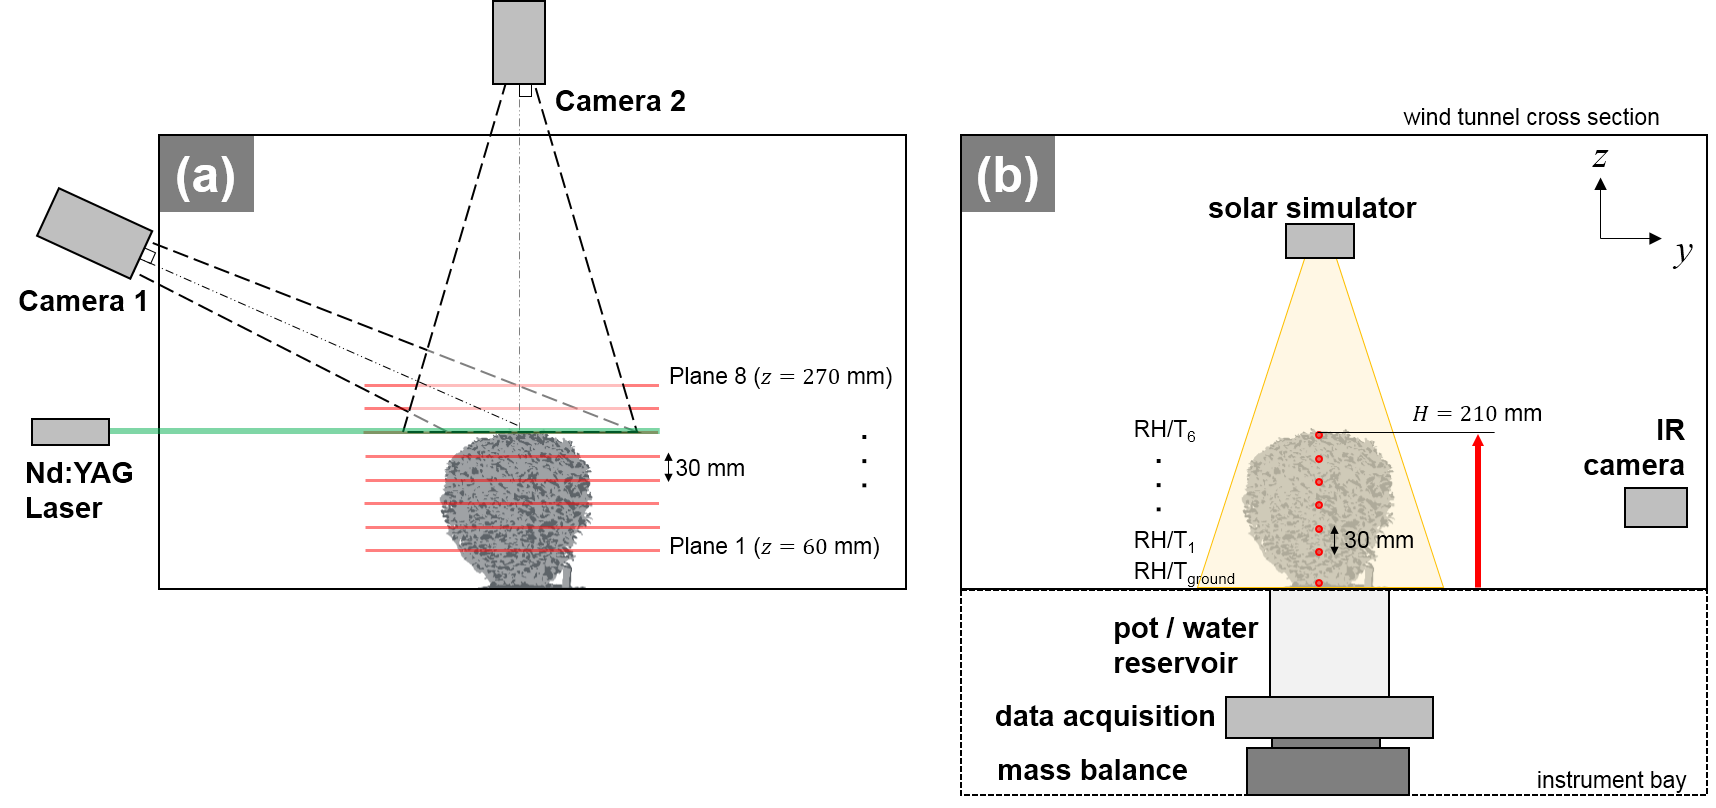
\includegraphics[width=\textwidth]{\figdir/fullsetup.png}
		\caption{Wind tunnel setup used to measure the  airflow and microclimate of the plant: \subfig{a} A stereo-PIV setup for multi-plane time-averaged measured consisting of $8$ horizontal plane, $z=[60,90,120,150,180,210,240,270]$ mm, \subfig{b} A microclimate measurement setup consisting of solar simulator, IR camera and SHT sensors inside the wind tunnel, mass balance and other data acquisition system below the wind tunnel through an access panel. The two distinct setups are required for non-interfered optical measurement of the PIV.}
		\label{fig:fullsetup}
	\end{sidewaysfigure}
	%	\end{figure}
	
\subsubsection*{Microclimate and net transpiration rate measurement}
The microclimate and thermal measurements of the plant due to various wind conditions and radiation condition is investigated separately from the flow field PIV measurement, as shown in \cref{fig:fullsetup}. \cref{fig:fullsetup}b shows the setup used to measure the microclimatic interaction of the plant. The solar simulator is placed above the plant providing $100$ W~m$^{-2}$ of incident short-wave radiation at the plant-canopy ($H=210$ mm). The solar simulator is controlled using a timer switch that provides a 12-hour period of $0$ and $100$ W~m$^{-2}$ radiation, mimicking a simplified diurnal solar cycle. The net plant transpiration is measured using a Mettler PM6100 mass balance placed below the wind tunnel section in the instrument bay along with the plant reservoir and the data acquisition system, to minimize their inferences on the flow field. The mass balance has a maximum capacity of $6.1$ kg and provides a precision of $0.1$ g. Simultaneously, the humidity and temperature profiles inside and around the plant are measured using Sensirion SHT35 sensors placed as indicated in \cref{fig:fullsetup}b. The SHT sensors are placed as follows: 5 sensors are directly inside the foliage with a vertical offset of $30$ mm starting below the plant canopy, 1 sensor at plant canopy, 1 sensor directly downstream of the plant at the height of plant canopy, and finally, 1 sensor below the plant foliage near the ground, to measure the shaded conditions. Thus, a total of 8 SHT sensors with an accuracy of $\pm 1.5$\% RH (between $0$ and $80$\% RH) and $\pm 0.1$ $^{\circ}$C (between $20$ $^{\circ}$C and $60$ $^{\circ}$C) are used. The leaf temperatures are recorded using a pre-calibrated Type-T thermocouple taped to the outer leaves of the plant foliage, at various locations. To ensure uninterrupted transpiration from the leaves, permeable 3M Micropore surgical tapes are used. All the sensors for the plant are connected and powered by the wireless data acquisition system directly below the plant pot. The wireless data acquisition system consists of an Arduino Micro and a \num{20100} mAh powerbank providing the necessary power for a multi-day measurement period. The Arduino Micro serves not only as analog-to-digital signal converter but also a telemetry device for sending the acquired data to the data logger away from the measurement setup. This wireless data acquisition system configuration is necessary to obtain a valid transpiration-driven plant mass loss. The data is acquired at $30$ second interval. Simultaneously, the plant foliage temperature is measured using an IR thermography setup.

\subsubsection*{Infrared imaging}
An infrared (IR) thermography is performed to obtain a high-resolution spatial and temporal, quantitative understanding on the influence of foliage temperature to varying environmental conditions. Therefore, an IR imaging system is employed to measure the outer plant foliage temperature simultaneously with the microclimate and net transpiration rate measured for two different wind condition throughout the diurnal radiation cycle. The IR imaging system consists of the Optris PI 640 IR camera with a $640\times480$ px$^2$ sensor, a spectral response between $7.5$ and $13$ $\mu$m and set to measure $-20$ to $100$ $^{\circ}$C with an accuracy of $\pm2$ $^{\circ}$C \citep{Allegrini2018,Tsalicoglou2018}. A $33^{\circ}$ lens is used providing an effective FOV of $223\times211$ mm$^2$. The IR measurement is performed $1$ frame/minute throughout the full diurnal cycle. The infrared device, the SHT sensor and the thermocouples are aggregately calibrated with PT100 sensor (platinum resistance thermometer). A PT100 sensors is placed in FOV of the IR image for calibration \citep{Allegrini2018}. Additionally, the ground SHT sensor and a thermocouple is aggregated together in front IR camera, for cross-comparison of the measurement devices.


\section{Results and Discussion}

Firstly, the plant traits such as foliage geometry, porosity distribution, and leaf area are derived from the x-ray tomography \cref{subsec:xraytomo}. We show that such properties can be derived with the benefit of being a non-destructive and furthermore provides spatial resolution, which is not possible in other state-of-art techniques. Thereafter, the wake flow field resulting from the foliage heterogeneity is investigated using stereoscopic particle image velocimetry (Stereo-PIV), detailed in \cref{subsec:stereopiv}. The necessity of such a technique is verified from the 3D nature of the flow field. The influence of the heterogeneous porosity distribution and the 3D wake flow field on the plant behavior is investigated at two timescales: firstly, the diurnal response of the plant identifying daytime and nighttime averages (\cref{subsec:diurnal}); and secondly, identifying the dynamic responses of the plant resulted from the plant hysteresis that is seldom modeled in microclimate models with vegetation (\cref{subsec:dynamic}). 

\subsection{X-ray tomography: A non-destructive approach to obtain plant traits}
\label{subsec:xraytomo}

The x-ray tomographic approach is a non-destructive approach to obtain the high-resolution plant morphological traits. The detailed description of the X-ray imaging approach is provided in \textbf{section 2.2.1}. The reconstructed tomographic data provides the 3D distribution of X-ray attenuation by the sample, where the voxel intensities are given in Hounsfield units (HU):
\begin{equation}
\textit{HU} = 1000 \times \frac{\mu - \mu_{\textit{air}}}{\mu_{\textit{water}} - \mu_{\textit{air}} }
\end{equation}
and can be used to extract the biological properties of the plant. The Hounsfield scaling normalizes the measured attenuation coefficient $\mu$ with that of the air and distilled water at standard atmospheric conditions, where the attenuation coefficients of air and water are $-1000$ and $0$, respectively. Therefore, the scaling can be a means for fast and simple categorization of biological matter with different water quantity. \cref{fig:figure_rawimage} shows a single image slice at the middle of the volumetric dataset and \cref{fig:figure_rawimage} shows the associating histogram distribution. A preliminary observation of the images that the attenuation of air, leaf, and branch has a distinct regime, where the air voxels can be distinguished. Therefore, for an initial segmentation of leaf, air, and branches, a manual threshold of the histogram is performed. Afterward, to obtain a better segmentation, a supervised learning technique is employed.

\begin{figure}[t]
	\centering
	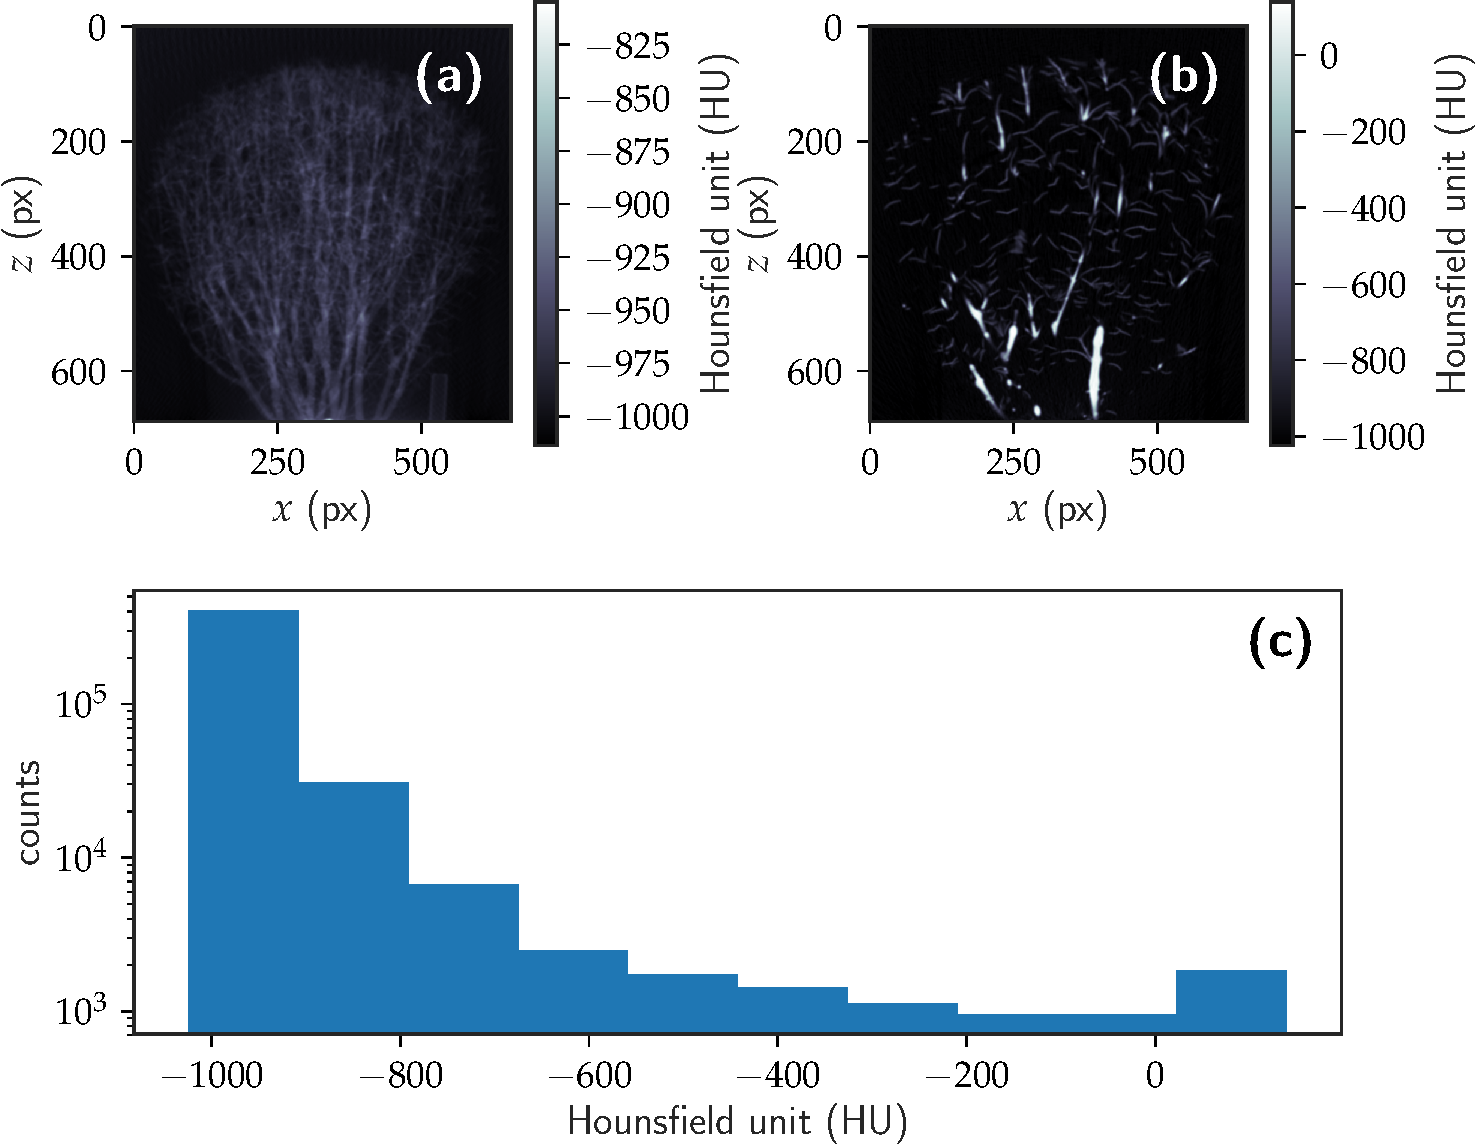
\includegraphics[width=\textwidth]{\figdir/figure_rawimage-crop.pdf}
	\caption{Raw image obtained from x-ray CT-scan: \subfig{a} Spatially-averaged ($y$-axis) plant attenuation, \subfig{b} A single image slice at the middle of the plant, \subfig{c} Histogram distribution of \subfig{b}. The intensity is obtained in Hounsfield units (HU) where $-1000$ corresponds to air and $0$ corresponds to pure water. The image slice resolution is $\Delta x = \Delta z=0.318$ mm with a slice thickness of $\Delta y=0.4$ mm.}
	\label{fig:figure_rawimage}
\end{figure}

\subsubsection*{Image segmentation}

To determine the spatial distribution of the leaves and branches, two different approaches are used. The first approach is based on simple histogram-based segmentation dividing the pixels of intensity into air ($-1000$ to $900$), leaves ($-900$ to $-700$), branches ($-700$ to $200$) and anything beyond as foreign material. The selection was based on user-defined visual cues and serves as a base-segmentation for comparison and validation of the more advanced approach. \cref{fig:xrayctslice}a shows the original dataset before the classification and \cref{fig:xrayctslice}b shows the histogram-based classification labels. A first observation shows a surprisingly good classification of the dataset except at boundaries of the branches. The boundaries of the branches are seen to be classified as leaves due to the diffused intensity at the boundaries. Therefore, there is an over-estimation of the leaf pixels using such simple segmentation.

	\begin{figure}[t]
		\centering
		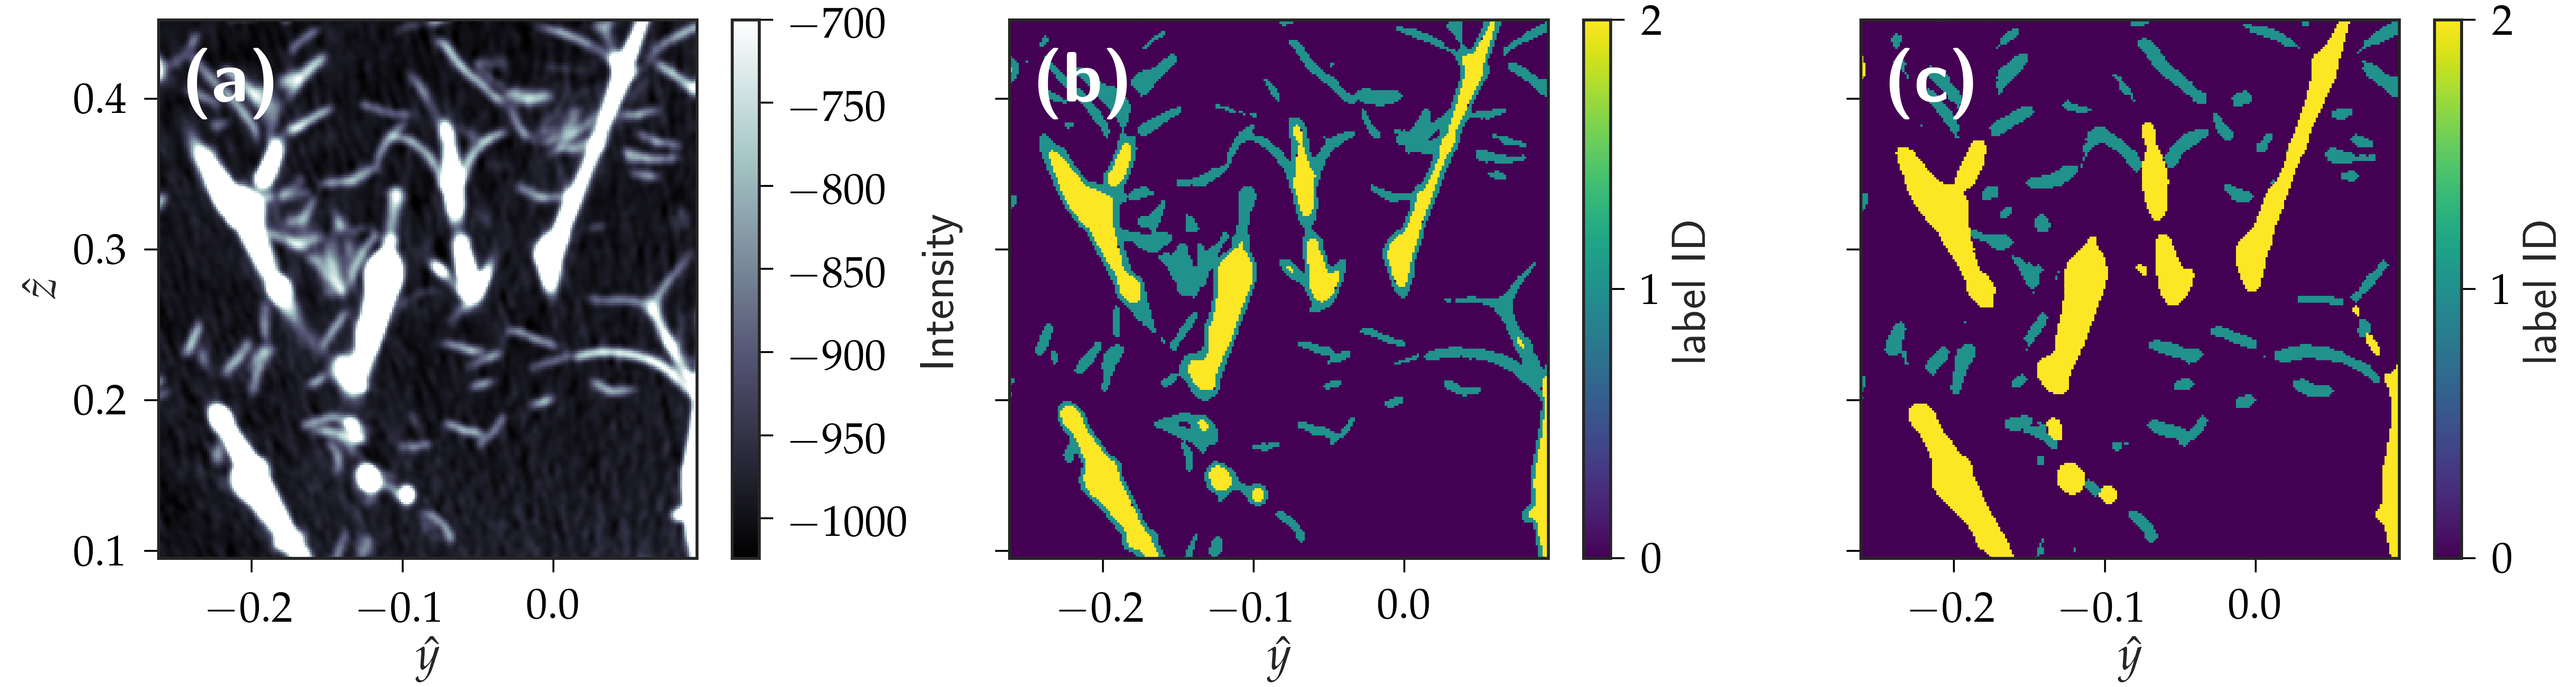
\includegraphics[width=\textwidth]{\figdir/figure_segentation_poster.png}
		\caption{Segmentation of the X-ray CT scan: \subfig{a} slice of original X-ray CT dataset, \subfig{b} segmentation using user-defined histogram threshold and \subfig{c} segmentation using trainable WEKA segmentation and additional morphological operation (opening $+$ closing). Only a sub-region of an image slice is shown for clarity. The segmented pixels are labeled as air: $0$, leaf: $1$ and branch: $2$.}
		\label{fig:xrayctslice}
	\end{figure}

Therefore, a more advanced approach such as the Trainable Weka Segmentation (TWS) \citep{Arganda-Carreras2017} and additional binary morphological operations are used for classification. The TWS segmentation employs an implementation of fast random forest ensemble classification algorithm in the \texttt{Fiji} application \citep{Schindelin2012a}. The classifier uses 200 decision trees with 2 random features. The training features consist of various filters applied to the original dataset, consisting of Gaussian blur, Sobel filter, pixel-wise Hessian matrix, difference of Gaussians filter, mean filter, variance filter, anisotropic diffusion filter, Laplacian filter, entropy filter, and Neighbors filter. A larger selection of edge-enhancement filters is used to reduce the over-estimation of the leaves at the boundary. The training procedure consisted of providing an initially labeled training dataset, trained using the classier, visually validating the classification, and improving the user-provided labeled training dataset for improved classification. Finally, any small remaining leaf pixels at the boundary of the branches were removed using the binary opening and closing morphological operation using a python library, \texttt{scikit-image} \citep{VanderWalt2014a}. \cref{fig:xrayctslice}c shows the resulting segmentation using the decision tree classification and morphological operation. The figure shows a better classification of the plant elements and thereafter, a 3D surface of the branch and leaves are generated and verified. Therefore, from the segmented dataset, plant properties such as porosity distribution and the net surface area of the leaf can be estimated. 

\subsubsection*{Porosity distribution} 

To calculate the porosity distribution of plant, a valid representative element volume size has to be chosen to represent the plant foliage as a porous media. \cref{fig:porositydistribution}a shows the average porosity for voxel size ranging from $5$ to $100$ px$^3$. The average plant porosity is converged once a sufficiently large REV prescribed. However, a too large REV can reduce the porosity distribution resolution. Therefore, in our case, a REV size of $30$ px$^3$ is seen to be optimal provide sufficient accuracy of average porosity and sufficient spatial resolution. The resulting average plant porosity is $\phi= 0.881$. 

	\begin{figure}[p]
		\centering
		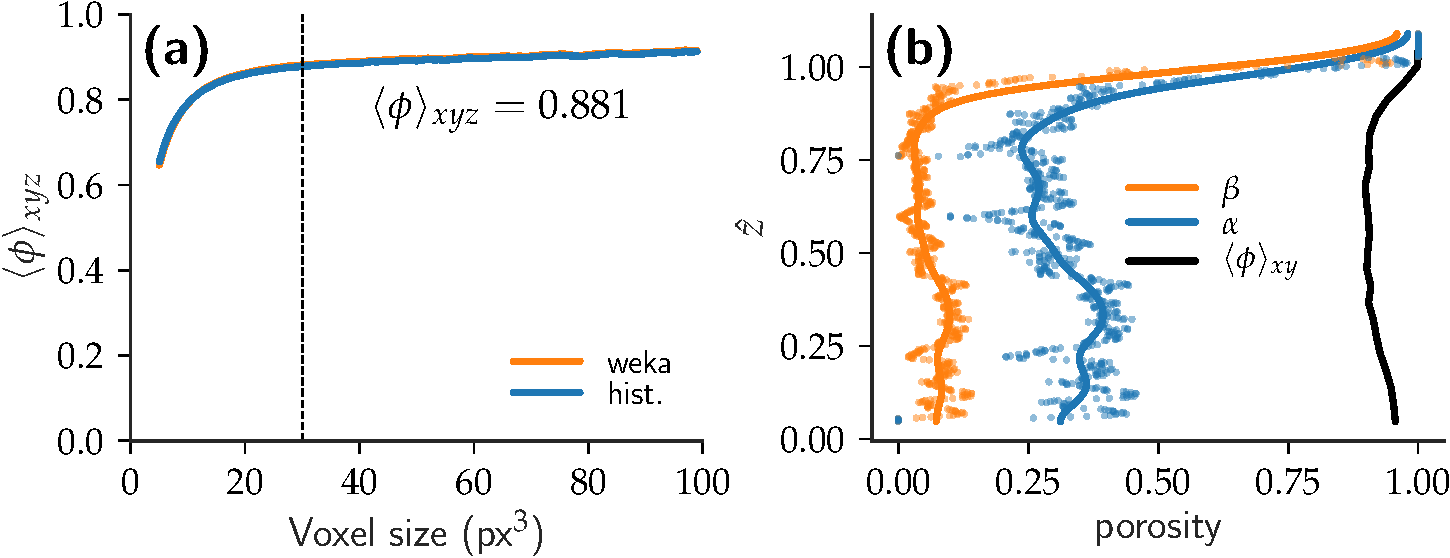
\includegraphics[width=\textwidth]{\figdir/porosity_verticaldistribution-crop.pdf}
		\caption{Determining the representative elementary volume for calculating porosity distribution: \subfig{a} Convergence of average plant porosity $\langle \phi \rangle_{xyz}$ with respect to voxel size (px$^3$) and \subfig{b} Various vertical porosity distribution: optical $\beta$, aerodynamic $\alpha$ and true porosity $\langle \phi \rangle_{xy}$.}
		\label{fig:porositydistribution}
	\end{figure}

	\begin{figure}[p]
		\centering
		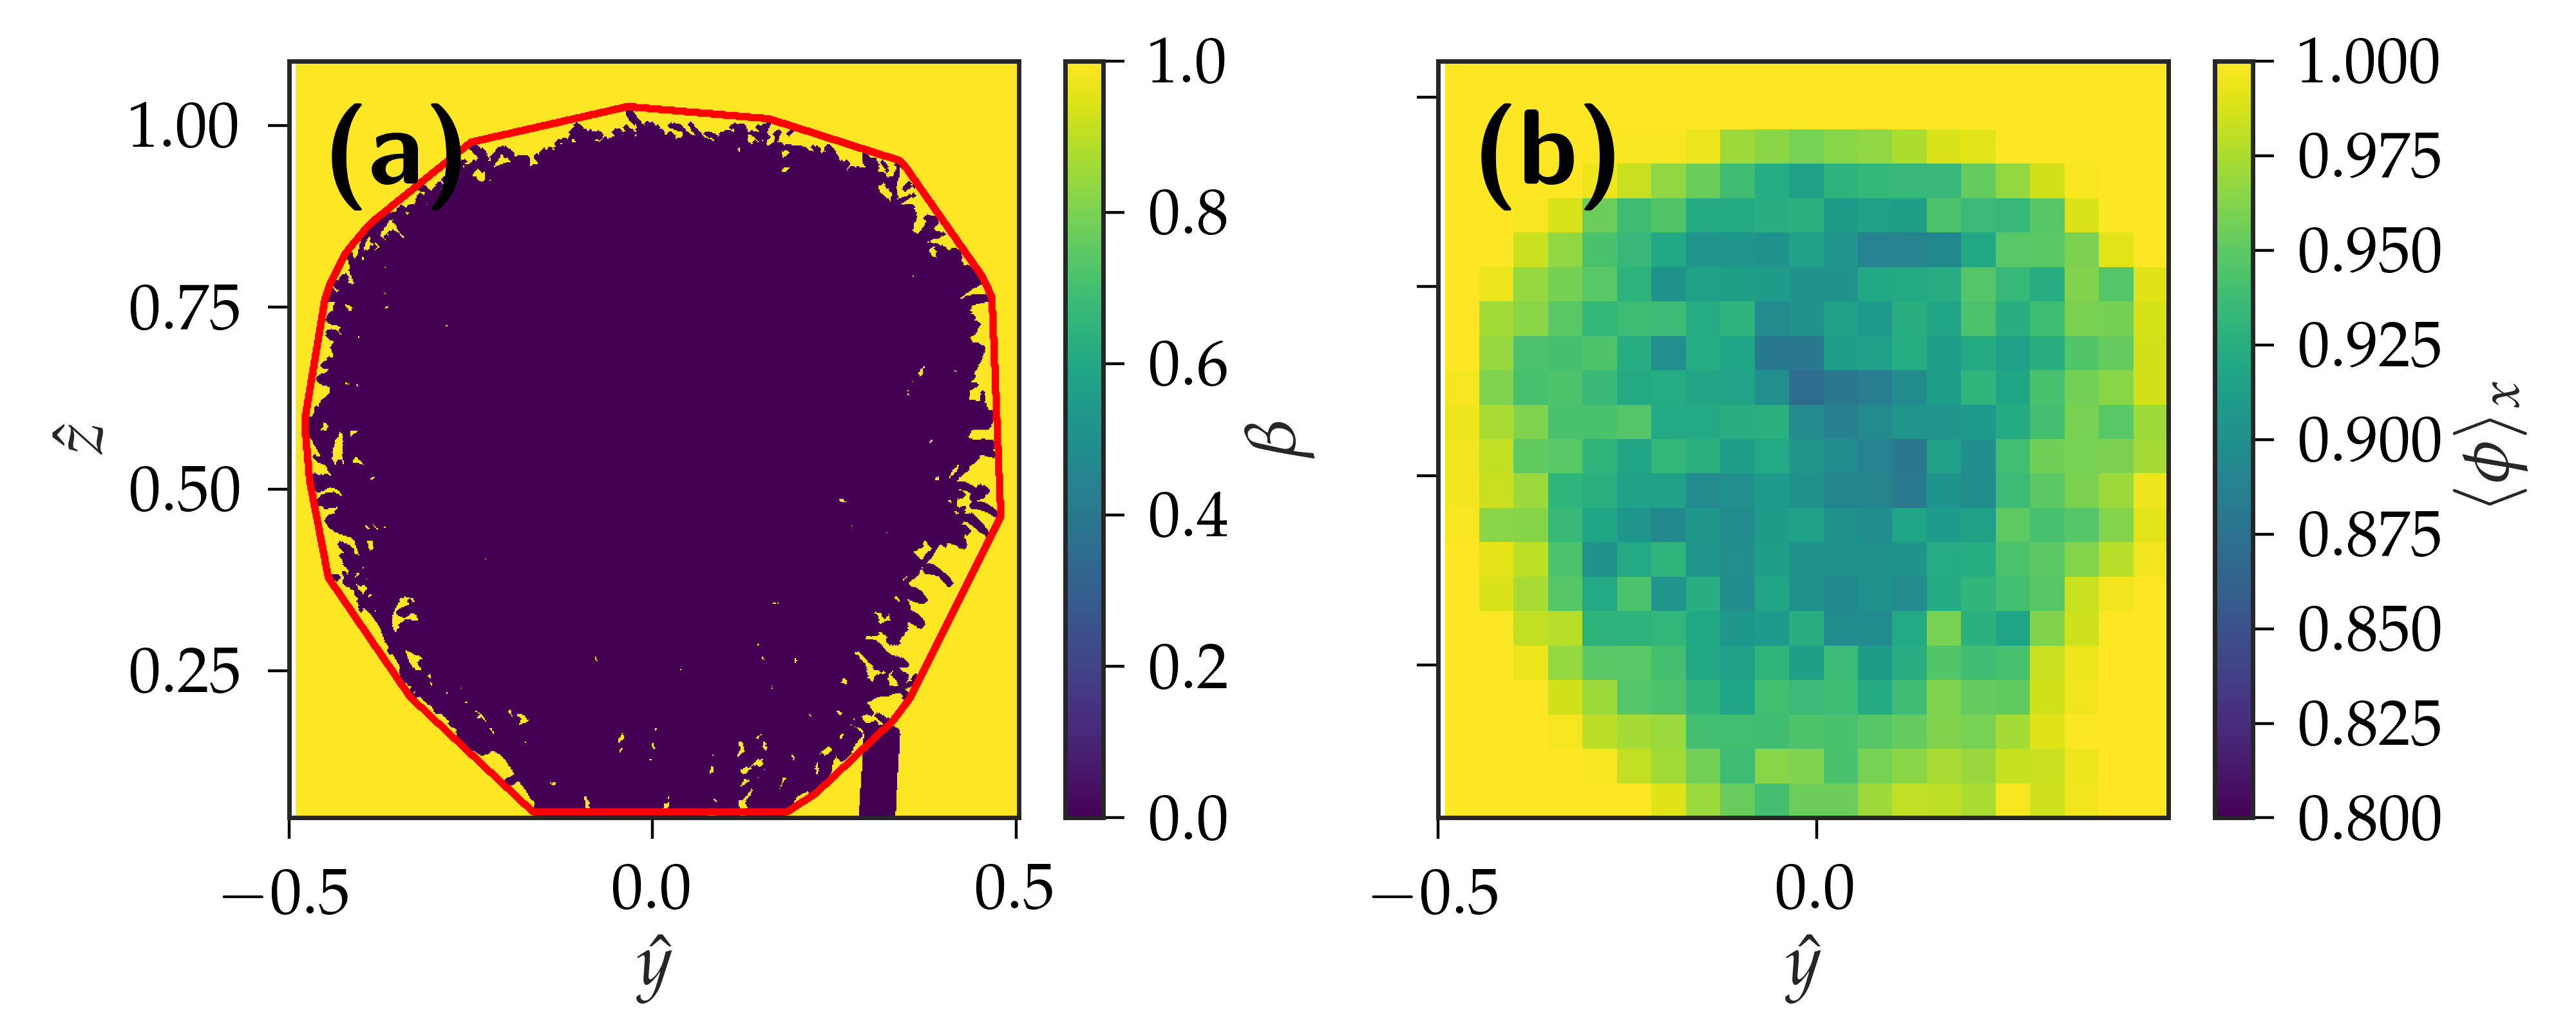
\includegraphics[width=\textwidth]{\figdir/optical_aerodynamic_true_porosity_distribution_type2.png}
		\caption{Porosity distributions of the plant: \subfig{a} The optical porosity $\beta$ with plant element and airspace indexed as $0$ and $1$, respectively and \subfig{b} streamwise-averaged plant porosity $\langle \phi \rangle_x$. }
		\label{fig:porosities}
	\end{figure}

\cref{fig:porositydistribution}b shows the vertical distribution of various porosities. In conjunction with the measured plant porosity (black line), the optical of the plant (with respect to the incident airflow in wind tunnel) is investigated. The optical and the aerodynamic porosity derived from this, are a typical measure used in the wind tunnel studies to estimate the aerodynamic contribution of the plant porosity \citep{Grant1998, Guan2003, Manickathan2018b}. The optical porosity $\beta$ and the aerodynamic porosity $\alpha$ are related as follows:
\begin{equation}
\alpha = \beta^{0.4}
\end{equation}
and in an empirical relationship. The optical porosity is obtained from a 2D optical image of the tree incident to the flow (\cref{fig:porositydistribution}a) and is defined as the ratio of empty pixels (without plant elements) to the total number of pixels within the silhouette of the plant, shown in  \cref{fig:porosities}a. A convex hull is used to define the silhouette of the plant. Furthermore, the streamwise-averaged plant porosity is investigated to quantify the amount of plant elements that will block the flow field at a given location, as shown in \cref{fig:porositydistribution}b. It indicates clearly that the highest blockage is found at the higher-middle region on the plant. Such location of high plant foliage density could indicate high solar radiative absorptions and a resulting high transpiration rate. A measure of the climatic conditions such as air temperature and relative humidity could indicate this hypothesis and show the regions of high transpiration. The plant foliage density is seen to reduce towards to the edges gradually and at these regions, a lower blockage might be present with a higher bleed flow. Furthermore, at locations with the higher bleed flow can provide internal ventilation, increasing the convective dominated processes such as sensible and latex heat flux \citep{Manickathan2018a}. Investigating the plant wake flow can, therefore, provide a better indication of the impact of the heterogeneity in the porosity distribution.

The horizontal-averaged ($x-y$ plane) porosity distribution is shown and compared in \cref{fig:porosities}b. Comparing optical, aerodynamic and true porosity, we see that the true porosity of the plant is substantially higher than the optical and the aerodynamic porosity, especially away from the plant canopy. Therefore, the flow field study can additionally indicate the efficacy of employing aerodynamic porosity vs. true plant porosity on quantifying the sheltering effect of the plant. 

\subsubsection*{Plant surface mesh and total leaf area}

\begin{figure}[t]
	\centering
	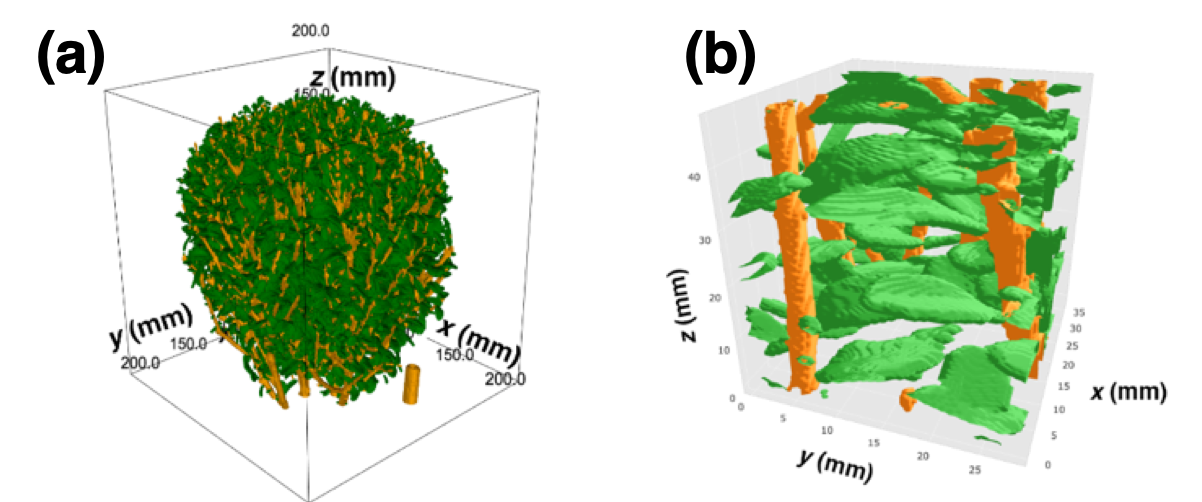
\includegraphics[width=\textwidth]{\figdir/plantmesh.png}
	\caption{Surface geometry of the plant, where leaves (green) and branches (orange) are differentiated: \subfig{a} complete plant surface, \subfig{b} sub-volume inside the plant foliage.}
	\label{fig:plantmesh}
\end{figure}

In addition to the porosity distribution of the plant, the total leaf area and the resulting leaf area index and leaf area density are important parameters for understanding and modeling the influence of vegetation \citep{Manickathan2018a}. The benefit of X-ray tomography is further evident as this parameter can not only be obtained using is a non-destructive but is also an accurate approach to estimate the spatial variability. Typically, the leaf area index (or density) is measured simply from optical measurements or by defoliating the entire plant \citep{Guan2003,Jonckheere2004,Manickathan2018b}. In our study, these plant traits are directly obtained from the x-ray tomography. To achieve this, the surface of the plant elements is generated from the volumetric data of the plant X-ray CT. \cref{fig:plantmesh}a shows the leaf and branch surface colored as green and orange, respectively. \cref{fig:plantmesh}b shows an internal sub-volume of the plant for clarity, and it is observable that the classification has been successful. The surface geometry is generated using a marching-cube algorithm implemented in \texttt{scikit-image} \citep{VanderWalt2014a}.

The total leaf surface area is simply the integral of the surface measure and is calculated to be $A_l=0.75$ m$^2$. A more general measure that is used to qualitatively and quantitatively indicate the amount of leaves is the leaf area index (LAI). The leaf area is defined as the ratio of one-sided leaf area the plant ground cover area:
\begin{equation}
\textit{LAI} = \frac{A_{\textit{l,one-sided}}}{A_g}
\end{equation}
The one-sided leaf area is simply half the total measured leaf area, and the plant ground cover area is obtained directly from the X-ray CT dataset. The plant ground cover was also determined to be $A_g=0.031$ m$^2$, and a resulting leaf area index of $LAI=12.14$ m$^2$~m$^{-2}$ is measured. Thus, an average leaf area density of $LAD=57.79$ m$^2$~m$^{-3}$ for a plant height of $H=210$ mm.

\subsection{Stereoscopic Particle Image Velocimetry: 3D wake flow characterization }
\label{subsec:stereopiv}

To study the influence of the plant morphology, measured through X-ray tomography in \cref{subsec:xraytomo}, on the flow field, a stereoscopic particle image velocimetry (Stereo-PIV) approach is employed. Furthermore, to study the resulting 3D wake flow field of the plant and the impact of heterogeneous porosity distribution, the stereo-PIV system measures multiple horizontal planes to capture the full time-averaged plant wake. The setup of the PIV system is detailed in \cref{subsec:windtunnelsetup}, measuring 8 horizontal planes behind the plant at vertical heights of $h =$ $[60$, $90$, $120$, $150$, $180$, $210$, $240$, $270]$ mm.

\subsubsection*{Normalized mean velocity magnitude}
	
\begin{sidewaysfigure}[p]
	\centering
	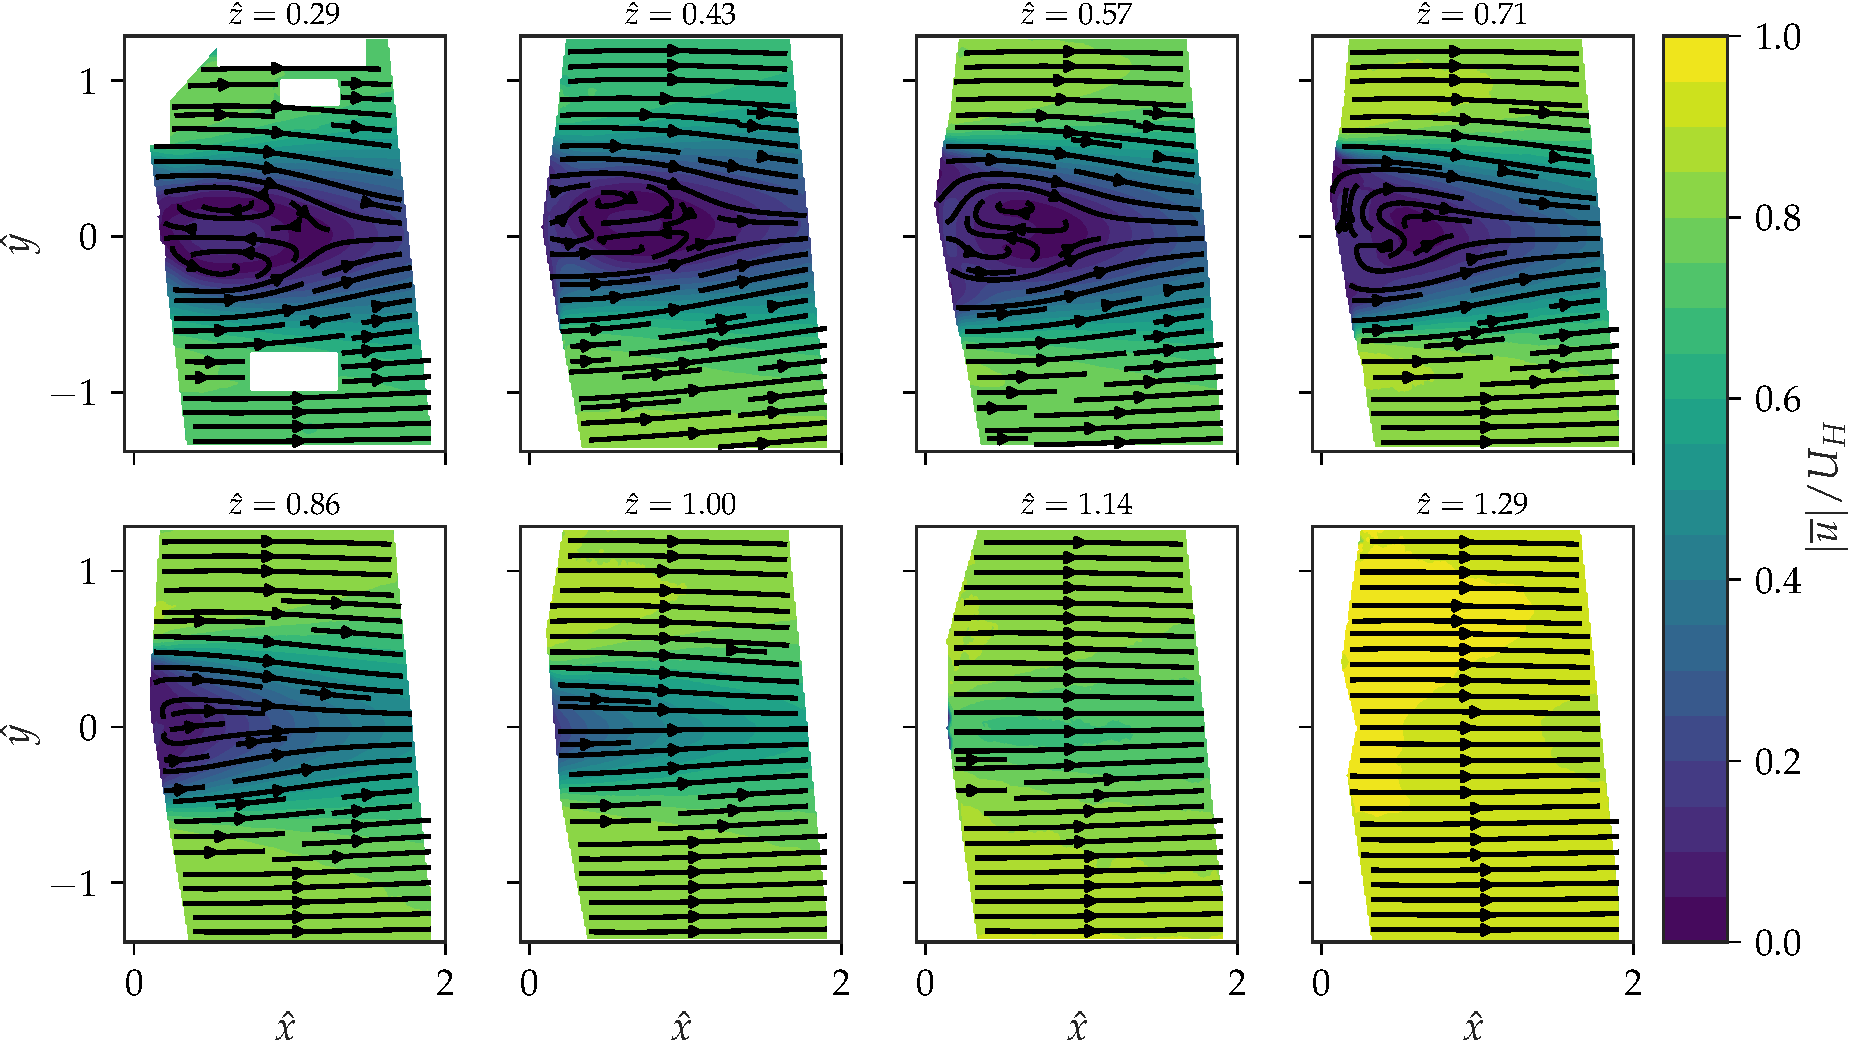
\includegraphics[width=\textwidth]{\figdir/hAll_velocitymagnitude-crop.pdf}
	\caption{Normalized mean velocity magnitude $\tavg{\mvec{u}}/U_H$ at 8 horizontal planes, $\hat{z}=$ [$0.29$,~$0.43$,~$0.57$, $0.71$, $0.86$, $1.0$, $1.14$, $1.29]$.}
	\label{fig:meanflow}
\end{sidewaysfigure}

The measurement planes up to a height of $210$ mm are directly in the wake, and the last two heights measure the above-canopy zone. The goal of these exhaustive measurements is to quantify the spatial variability of the plant wake and the 3D nature of the flow generated from the isolated plant. \cref{fig:meanflow} shows the normalized mean velocity magnitude $|\tavg{\mvec{u}}|/U_H$. The coordinate system is normalized with the tree height of $H=210$ mm, where $\hat{x}_i = x_i / H$ for $x_i =\{x,y,z\}$. The mean velocity distribution shows a prevailing recirculation flow for $\hat{x} \le 0.71$, which indicates a wake flow with low bleed-flow. However, further above the tree, the wake flow structure is indicative of bleed-flow showing non-circulating streamlines. Once we investigate the vertical porosity distributions, \cref{fig:porosities}b, we realize that above $\hat{z}>0.71$, the porosity distribution quickly increases to $\phi=1$, correlating the observed bleed-flow from PIV measurement. To further study the impact of such flow configuration on the climate, the influence of the flow conditions on the microclimate inside the plant must be investigated (\cref{subsec:diurnal}). 


\subsubsection*{Turbulent kinetic energy budget}
		
	\begin{sidewaysfigure}[p]
		\centering
		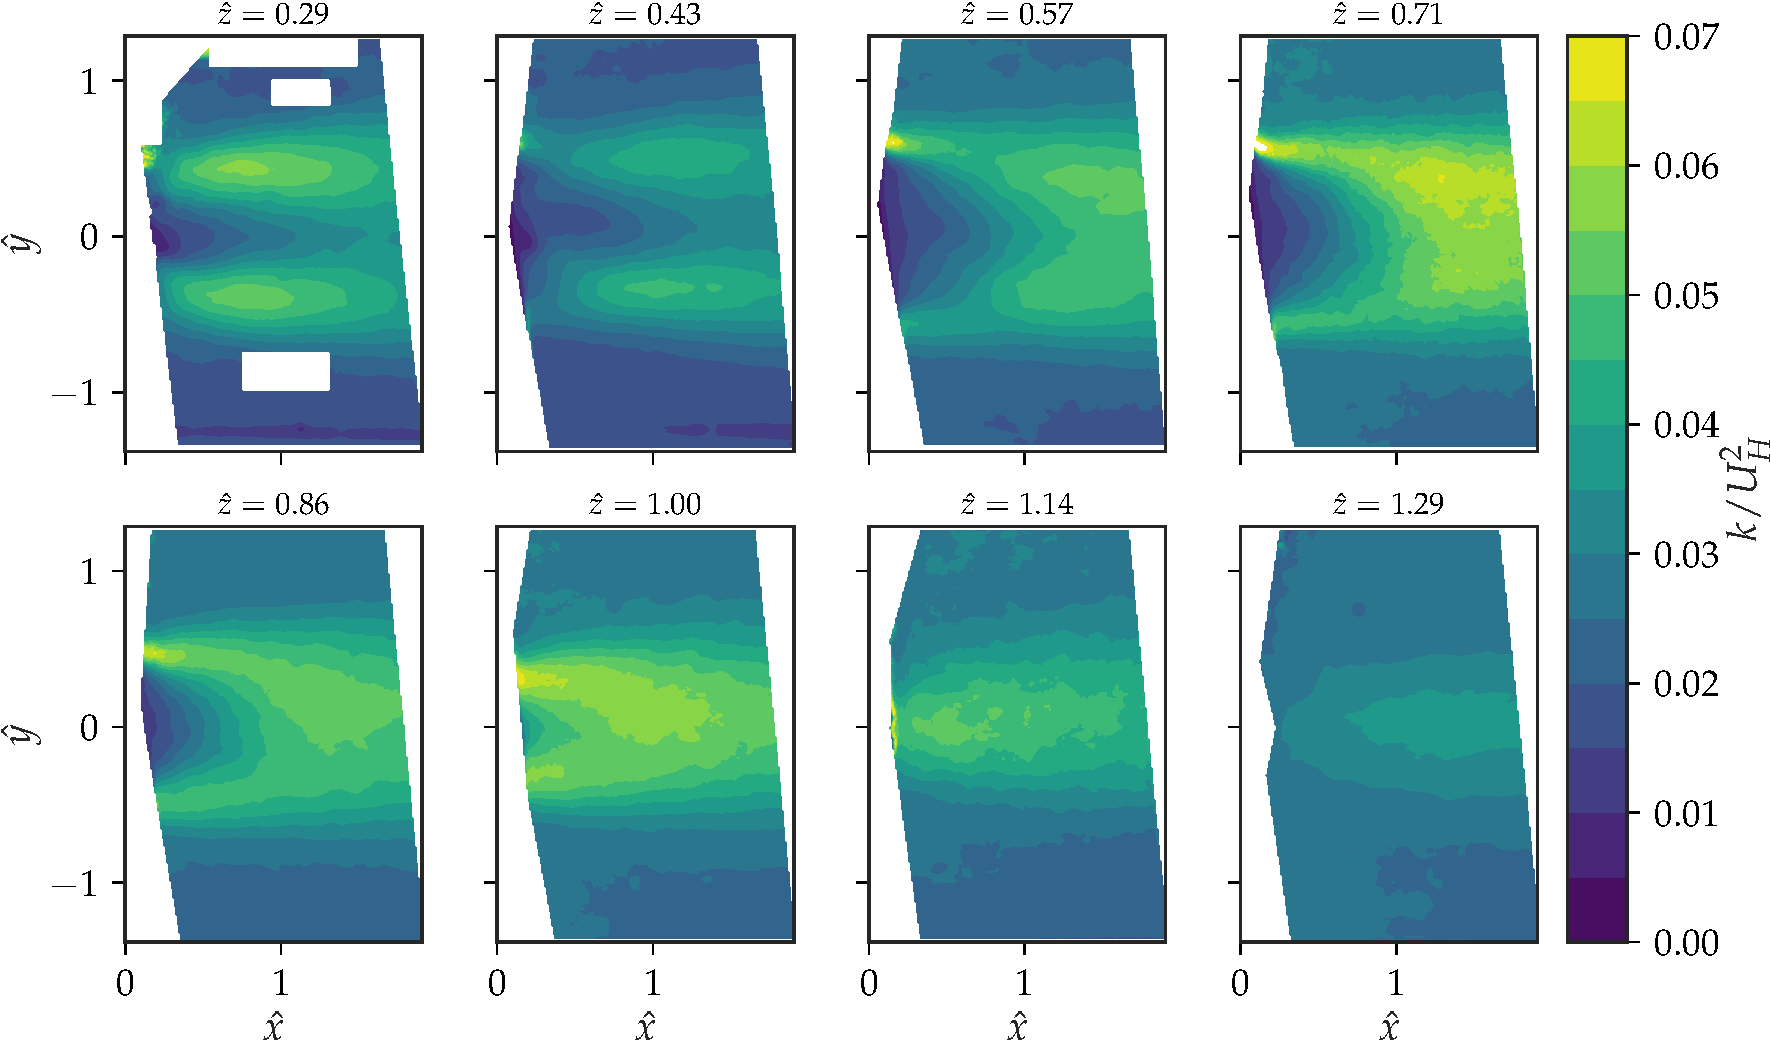
\includegraphics[width=\textwidth]{\figdir/hAll_TKE-crop.pdf}
		\caption{Normalized turbulent kinetic energy $k/U_H^2$ at 8 horizontal planes, $\hat{z}=$ [$0.29$,~$0.43$,~$0.57$, $0.71$, $0.86$, $1.0$, $1.14$, $1.29]$.}
		\label{fig:tke}
	\end{sidewaysfigure}


A more important impact of trees of the air flow is the turbulence modification resulted from the plant porosity. In literature, several studies emphasize the role of vegetation in turbulence enhancement for urban flows, which can drastically influence of the pollution dispersion and thermal characteristics \citep{Amorim2013,Gromke2008,Poggi2004}. The spatial variability in the turbulent kinetic energy (TKE) of the plant wake is investigated to understand the turbulence modification due to the porosity distribution. \cref{fig:tke} shows the normalized turbulent kinetic $k/U_H^2$ for the 8 horizontal planes. Trivially, the TKE is minimal in the freestream region and directly behind the plant (near  $\hat{x}= 0, \hat{y} = 0$ mm), where the flow is laminar or stagnated, respectively. In contrast, the TKE is high right near the shear zones at the transition between high and low wind speeds. Comparing different planes, we see that the TKE profile is high near the ground ($\hat{z}=0.29$) and near the plant canopy ($\hat{z}=1$). This again is attributed to the high shear flows generated from the boundaries of the plant foliage that is present at these two vertical levels. The exception to this a quantifiably high TKE regions for the vertical plane $\hat{z}=0.71$. Investigating, the vertical porosity of plant, \cref{fig:porosities}b, a dip in plant porosity is observed. Therefore, the increases in the TKE can result from the sudden variability in plant porosity, and we see the impact of porosity heterogeneity on the mixing characteristics.

\subsubsection*{Influence of porosity on wake turbulence}
	
	\begin{figure}[t]
		\centering
		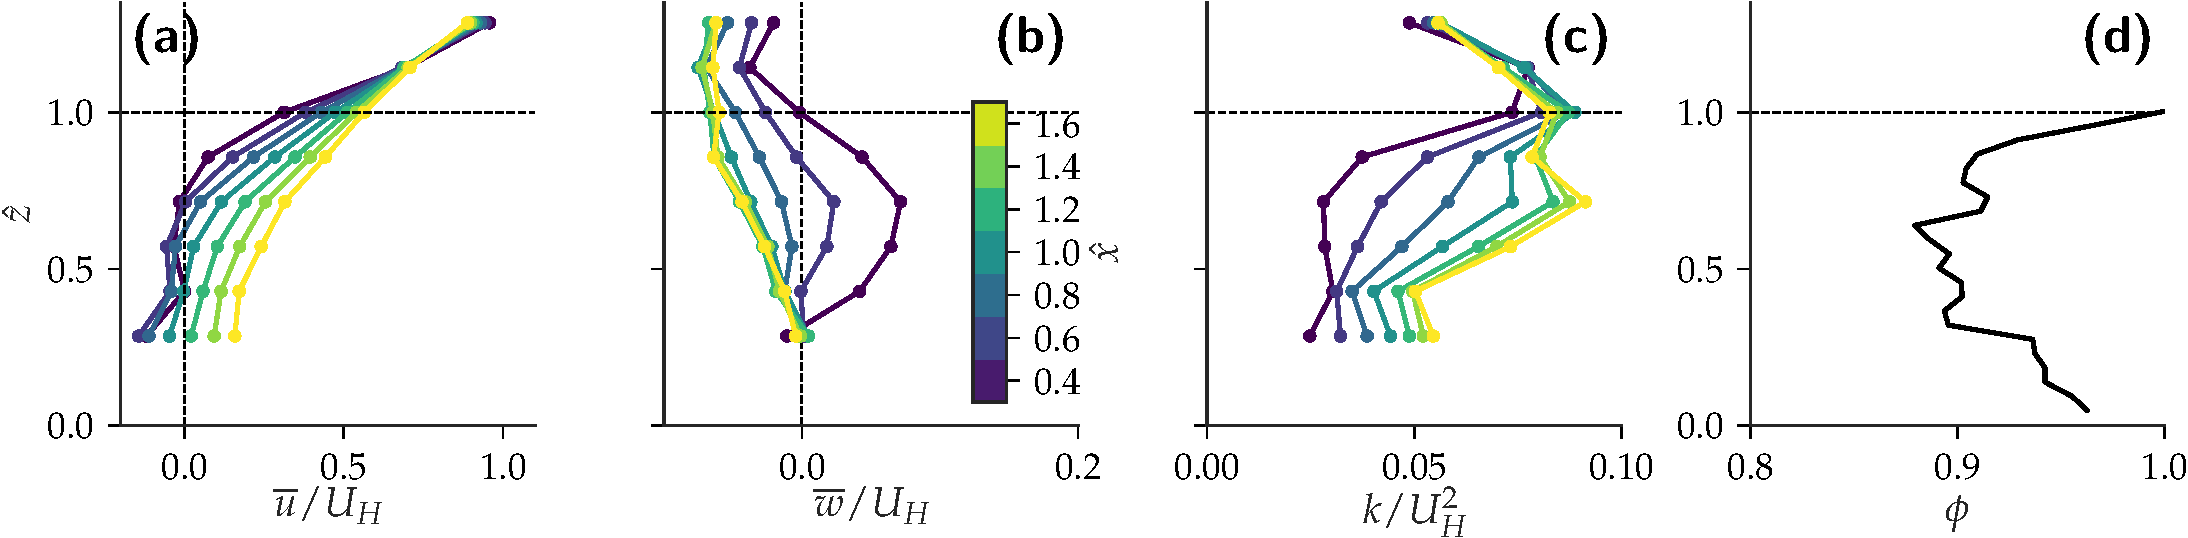
\includegraphics[width=\textwidth]{\figdir/figure_velocityprofile_centerline-crop.pdf}
		\caption{Mean vertical profiles at 7 streamwise positions $\hat{x}$ at center-line of the plant $\hat{y} = 0$: \subfig{a} streamwise velocity $\tavg{u}/U_H$ \subfig{b} vertical velocity $\tavg{w}/U_H$, \subfig{c}  turbulent kinetic energy $k/U_H^2$ and \subfig{d} streamwise-averaged porosity $\langle \phi \rangle_x$.}
		\label{fig:verticalprofile}
	\end{figure}

To better study the influence of plant porosity on the wake profile, the centerline flow statistics, and the plant porosity is compared in conjunction. \cref{fig:verticalprofile} shows the vertical profiles of the center-line velocity for 7 streamwise positions, $\hat{x} =$ $[0.4$, $0.6$, $0.8$, $1.0$, $1.2$, $1.4$, $1.6]$. At the vicinity of the trees and towards the lower half of the plant, the streamwise velocity $\tavg{u}$ is predominately negative. Furthermore, a positive vertical velocity $\tavg{w}$ is observed. This indicates a zone of strong circulation with reverse-flow configuration. Further downstream of the plant ($\hat{x}>0.8$), the streamwise velocity becomes positive and the vertical velocity becomes negative. Therefore, the flow characteristics is dominated by strong downwash of wind, bring high momentum velocity from above the plant canopy towards lower momentum regions of the ground. As such, the region is beyond the recirculation zone of the plant. The influence of porosity vertical variation on the mean velocities is not evident indicating no apparent correlation. However, the TKE profiles, especially away from the plant, shows a slight increase in TKE where the plant porosity is lower.

\subsection{Diurnal behavior of the plant}
\label{subsec:diurnal}

A thorough understanding of the plant morphology from section 3.1 and the resulting flow characteristics in \textbf{section 3.2} enables us now to obtain an understanding of the impact of the plant on the microclimate. The diurnal response of the plant and its daytime and nighttime averages are investigated. Thereafter, the dynamic characteristics during the transition between day and night are investigated. 

\subsubsection*{Influence of environment on diurnal response}

The diurnal behavior of the plant is investigated for two distinctly different boundary condition: no wind condition and wind condition with $U_{ref}=1$ m~s$^{-1}$. \cref{fig:figure_transpirationrate} shows the diurnal variation of the water mass loss $m$ (g) throughout the day and night and the resulting the transpiration rate $TR$ (g~h$^{-1}$), defined as:
\begin{equation}
TR = \frac{\mathrm{d}m}{\mathrm{d}t}
\end{equation}
measuring the hourly change in mass due to transpiration. We observe that during the night, regardless of the wind condition, a constant transpiration rate of $2.5$ g~h$^{-1}$ exists. This transpiration rate, at the absence of solar radiation, is therefore associated to water loss simply due to respiration \citep{Farquhar1980, Lambers2008, Launiainen2015}. At dawn, a stark increase in transpiration rate is observable. Furthermore, at this time, the wind condition plays an important role as during wind condition, a peak transpiration rate of $15$ g~h$^{-1}$ is observed. Whereas, without wind, the transpiration rate peaks only at $10$ g~h$^{-1}$. This dynamic response results from the delay in stomatal response. A detailed investigation of this hysteresis is presented in \cref{subsec:dynamic}. As the day progresses, the stomatal regulation is seen to compensate the influence of wind, resulting in similar transpiration rate with an average transpiration rate of $9$ g~h$^{-1}$. However, by the course of the day, the transpiration is seen to decay quantifiably. Such decay in the daytime transpiration rate has also been observed previously \citep{Javaux2013, Tuzet2003}. The phenomenon is attributed to the reducing rhizosphere soil moisture. The reduced soil moisture eventually reduces the stomatal conductance, resulting in the decayed transpiration rate that we observe. However, at night, the soil moisture equilibrates as the root water uptake is drastically diminished to only $2.5$ g~h$^{-1}$. 

	\begin{figure}[t]
	\centering
	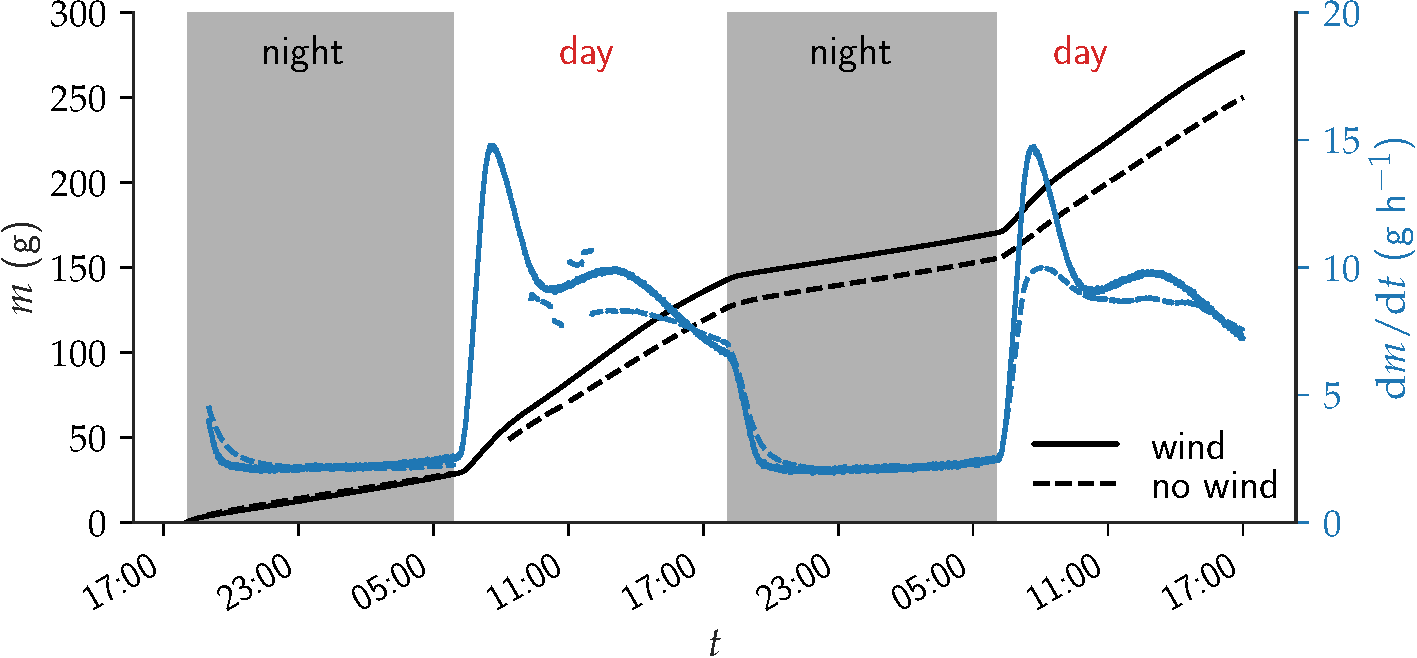
\includegraphics[width=\textwidth]{\figdir/figure_transpirationrate-crop.pdf}
	\caption{Diurnal variation of mass loss $m$ (g) and the resulting transpiration rate $TR=\mathrm{d}m/\mathrm{d}t$ (g h$^{-1}$) for two wind conditions: \textit{no wind} and \textit{with wind} ($U_{ref}=1$ m~s$^{-1}$).}
	\label{fig:figure_transpirationrate}
	\end{figure}

The influence of the varying transpiration rate is further investigated by studying the microclimate variables, air temperature T ($^{\circ}$C) and relative humidity RH (\%) inside the plant foliage. The setup of the microclimate sensors is detailed in \cref{subsec:windtunnelsetup}. \cref{fig:figure_airtemperature_humidity_v2} shows the diurnal variation of the air temperature and relative humidity inside the tree at various heights, with $T_1$ at the bottom of foliage and $T_6$ at the plant canopy ($H=210$ mm). The configuration is such that probes 1 to 5 are directly inside the plant foliage with $30$ mm offset. Furthermore, the ambient condition (``\textit{air}'') and the ground condition below the plant (``\textit{ground}'') is compared to study the influence of plant shading. \textbf{Fig. 14} shows that in the no wind condition, there is a quantifiable drop in the air temperature and a substantial increase in the relative humidity, with peak $RH=75$\% during day time. During the night, vertical variability in a microclimate within the foliage is smaller but still noticeable. All the sensors inside the plant foliage shows an improved thermal condition with lower temperature during day and night. However, the sensor at plant canopy ($H=210$ mm), shows that air temperature is noticeable higher than the ambient condition. This indicates that the plant canopy region is strongly influence by the absorption of solar radiation, leading to higher leaf temperature and positive sensible heat flux, thereby heating up the air. Similar observation of positive sensible heat flux due to high solar radiation absorption have also been observed numerically \citep{Manickathan2018a}. However, in the shadow of the plant, we see that air temperature is lower than sunlight region. This could be attributed to the secondary cooling (i.e., the cooling due to the ground) as the shaded ground has less thermal energy. 

	\begin{figure}[t]
	\centering
	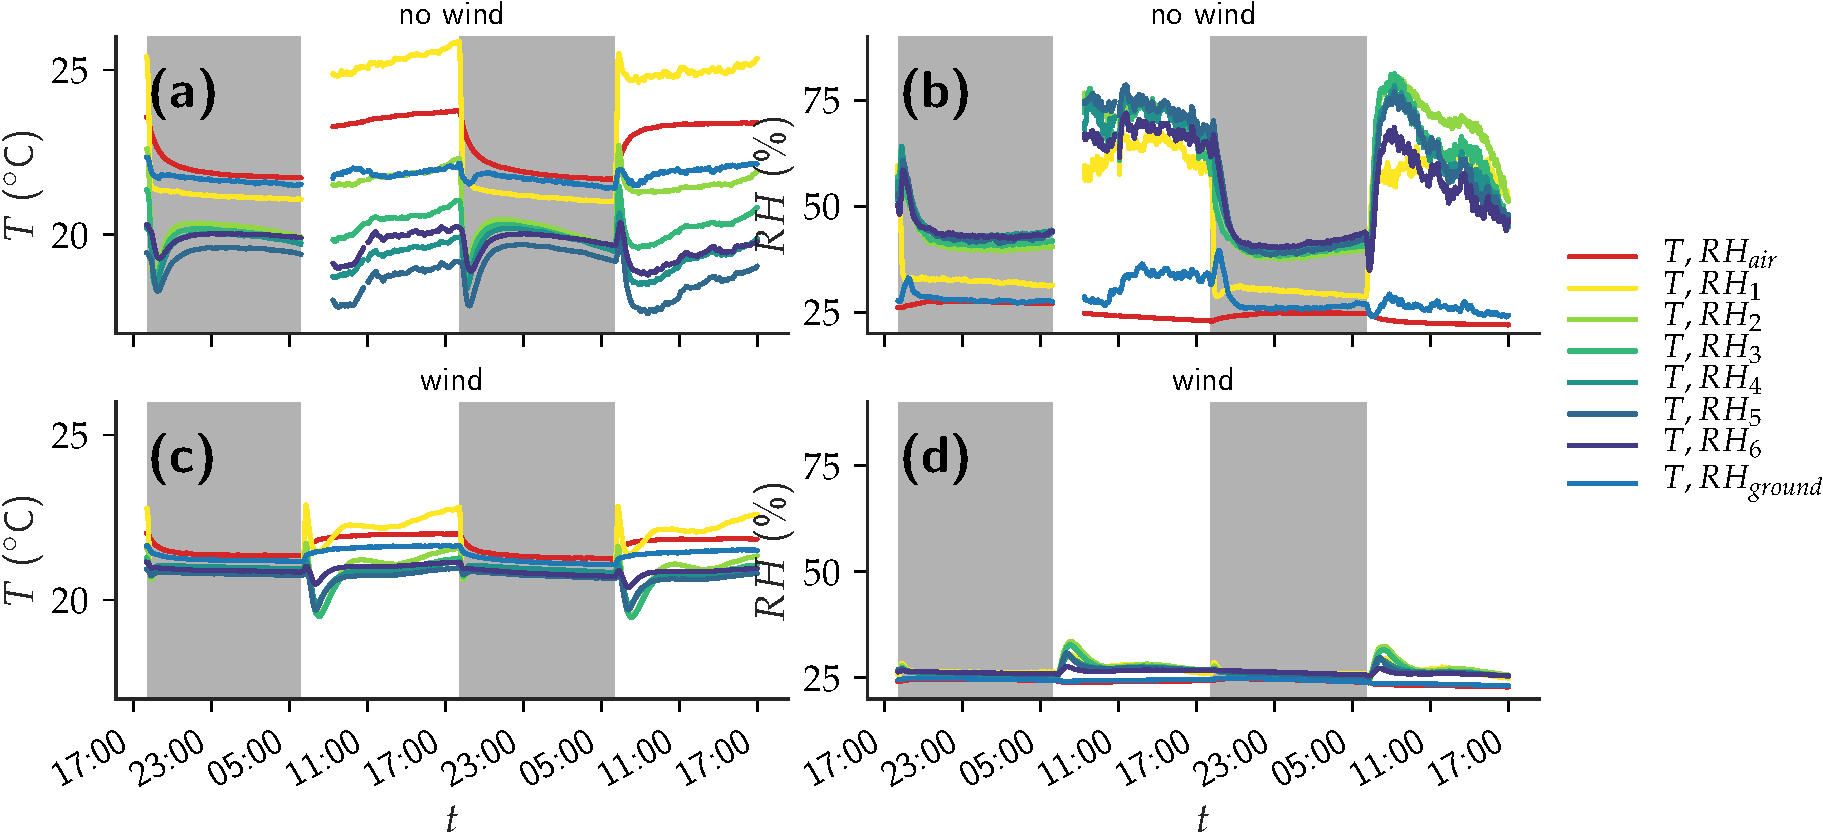
\includegraphics[width=\textwidth]{\figdir/figure_airtemperature_humidity_v2-crop.pdf}
	\caption{Diurnal variation of air temperature $T$ ($^{\circ}$C) and relative humidity $RH$ (\%) inside the tree at varying heights for two wind conditions: \subfig{a}\subfig{b} \textit{no wind} and \subfig{c}\subfig{d} \textit{wind} ($U_{ref}=1$ m~s$^{-1}$).}
	\label{fig:figure_airtemperature_humidity_v2}
	\end{figure}

The impact of transpiration of the microclimate is quickly diminished at the presence of wind. The wind conditions reduced the benefit of transpirative cooling due to increased ventilation of the plant foliage. Therefore, the maximum humidity within the plant is similar to ambient condition outside the plant. The influence of wind on transpiration rate is complex as we observed in \cref{fig:figure_transpirationrate}, the relative humidity inside the plant changes, the leaf temperature changes, and so, the vapor pressure gradient will also be different \citep{Manickathan2018a}. Furthermore, stomatal resistance is also a function of the VPD and so in our case transpiration rate is also affected. At dawn, we observe a large transpiration rate, however, by midday, equalizes to no wind condition. The observation is contrary to what is typically mentioned in literature, where the Penman-Monteith equation predicts a decrease in transpiration rate due to wind speed \citep{Dixon1983, Schymanski2016}. However, it is also mentioned that the type of species also has an influence \citep{Dixon1983}. 

\subsubsection*{Comparison of day and night plant response}

The average daily response of the plant and its influence on the climate is studied to understand the influence of vegetation. \cref{fig:figure_airtemperature_relativehumidity_profile} shows the median air temperature at various height for the case with wind and without wind, respectively. The figure furthermore differentiates the daytime and nighttime median air temperature. The figure shows, trivially, that the air temperature change is largest during the day. However, more interesting, the figure shows that during the wind case, the air temperature inside the tree is more homogenized, whereas, during the case of no wind, a large vertical variability is observable. Hence, we investigate the vertical heterogeneity in the air temperature and the relative humidity. We see that the most significant cooling, i.e., providing the largest drop in air temperature, is present for the no wind condition during the day for heights between $0.29\le\hat{x}\le0.57$. During this condition, we also observe a large increase in the relative humidity. During wind condition, and especially at night, the vertical variability in relative humidity and air temperature is diminished. This indicates that the cooling is only prevalent when transpiration is high and when the air is stagnated inside the plant, such that transpiration-driven cooling can effectively extract the thermal energy of the stagnated air. When, we investigate the influence of vertical porosity variation, we see no evident correlation on the thermal or moisture distribution. The key driving factor is the solar radiation intensity, which is highest at the plant canopy, and quickly decays into the foliage \citep{Manickathan2018a}. Such gradient in radiation absorption, results in the observed air temperature spike at plant canopy as indicated by sensor 6. The probes 1 to 5 that are within the foliage, which are protected from the solar radiation, shows a significantly lower air temperature.

	\begin{figure}[t]
	\centering
	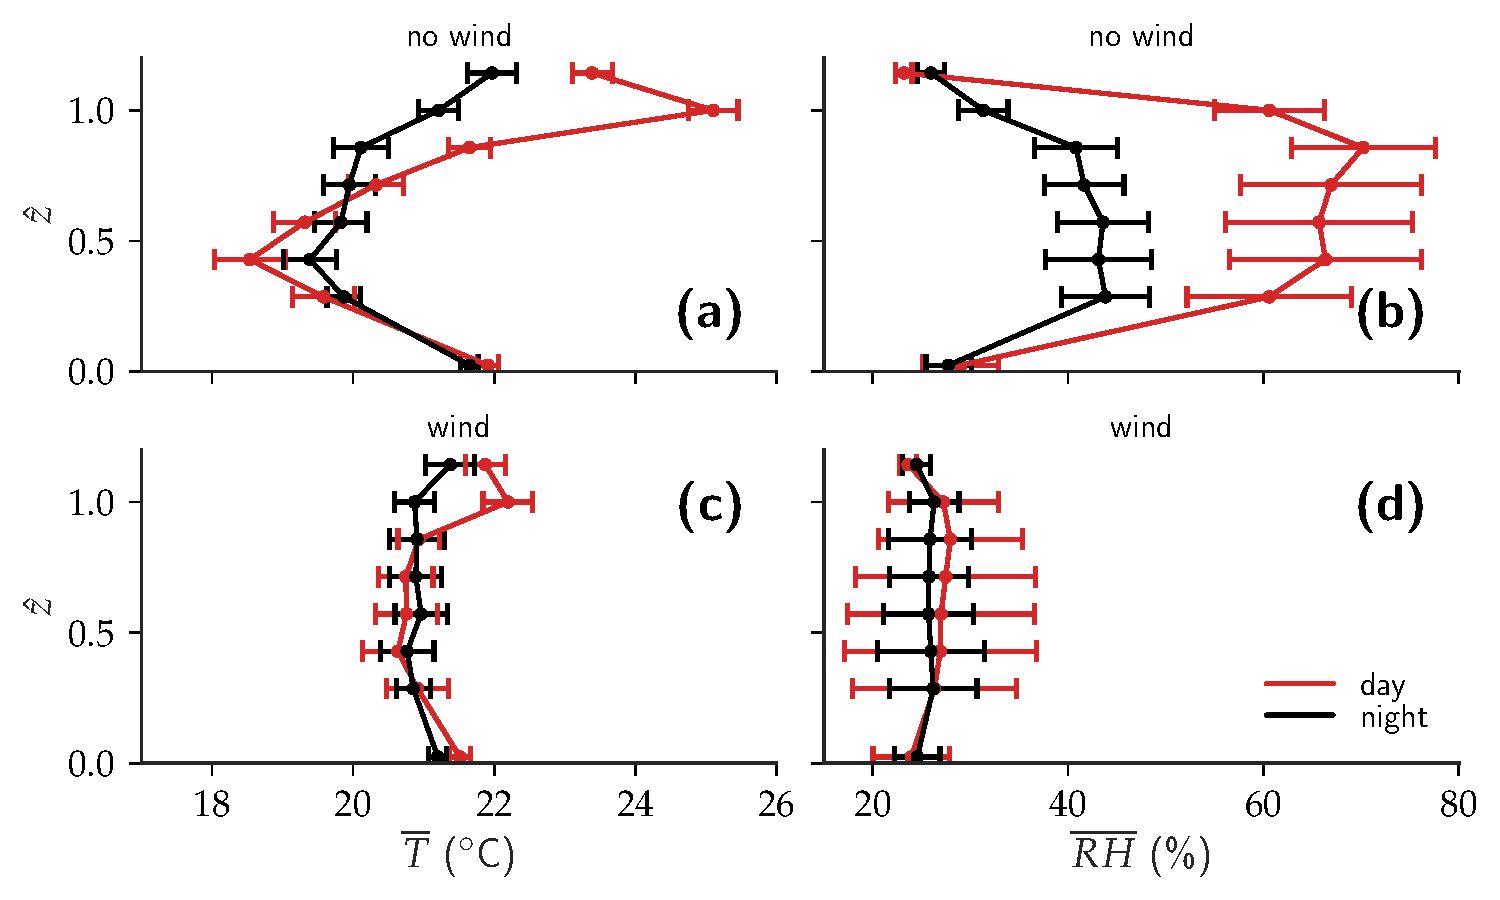
\includegraphics[width=\textwidth]{\figdir/figure_airtemperature_relativehumidity_profile.pdf}
	\caption{Mean vertical distribution of day (red) and night (black) \subfig{a}\subfig{c} air temperature $T$ ($^{\circ}$C) and \subfig{b}\subfig{d} relative humidity $RH$ (\%) inside the tree for two wind conditions: \subfig{a}\subfig{b} \textit{no wind} and \subfig{c}\subfig{d} with \textit{wind} ($U_{ref}=1$ m~s$^{-1}$).}
	\label{fig:figure_airtemperature_relativehumidity_profile}
	\end{figure}


To investigate the influence of transpiration on leaf temperature, the leaf temperature is measured through infrared thermography. \cref{fig:IR_dayvsnight_windvsnowind_type2_v2} shows the diurnal variation of leaf surface temperature for wind and no wind condition. The thermography shows that during the wind condition, the spatial variability in leaf temperature is minimal, especially during the night. Therefore, the convective exchanges equilibrate the leaf temperature variability arising from solar radiation. This is especially evident when observing the no wind condition. During the no wind condition, the vertical heterogeneity in leaf temperature is clear showing higher plant canopy leaf temperature and a cooler in foliage leaf temperature, especially at the lower regions. \cref{fig:IR_dayvsnight_windvsnowind_type2_v2}c and \cref{fig:IR_dayvsnight_windvsnowind_type2_v2}d shows the difference between the wind and no wind condition for night and day, respectively. During the night, the difference between no wind and wind condition is minimal with wind condition leaf temperature being slightly higher. Near the plant canopy, the leaf temperature difference for ``\textit{with wind}'' condition is substantially higher, indicating that when the wind is present, the leaf temperature is lower through the increased convective heat flux. The impact of higher leaf temperature is also reflected as previously observed in the air temperature,\textbf{ Fig. 15}. Moreover, the enhanced cooling observed during no wind condition during the day (\textbf{Fig. 15a}), is also reflected by the lower leaf temperature shown in \cref{fig:IR_dayvsnight_windvsnowind_type2_v2}d.

	\begin{figure}[t]
	\centering
	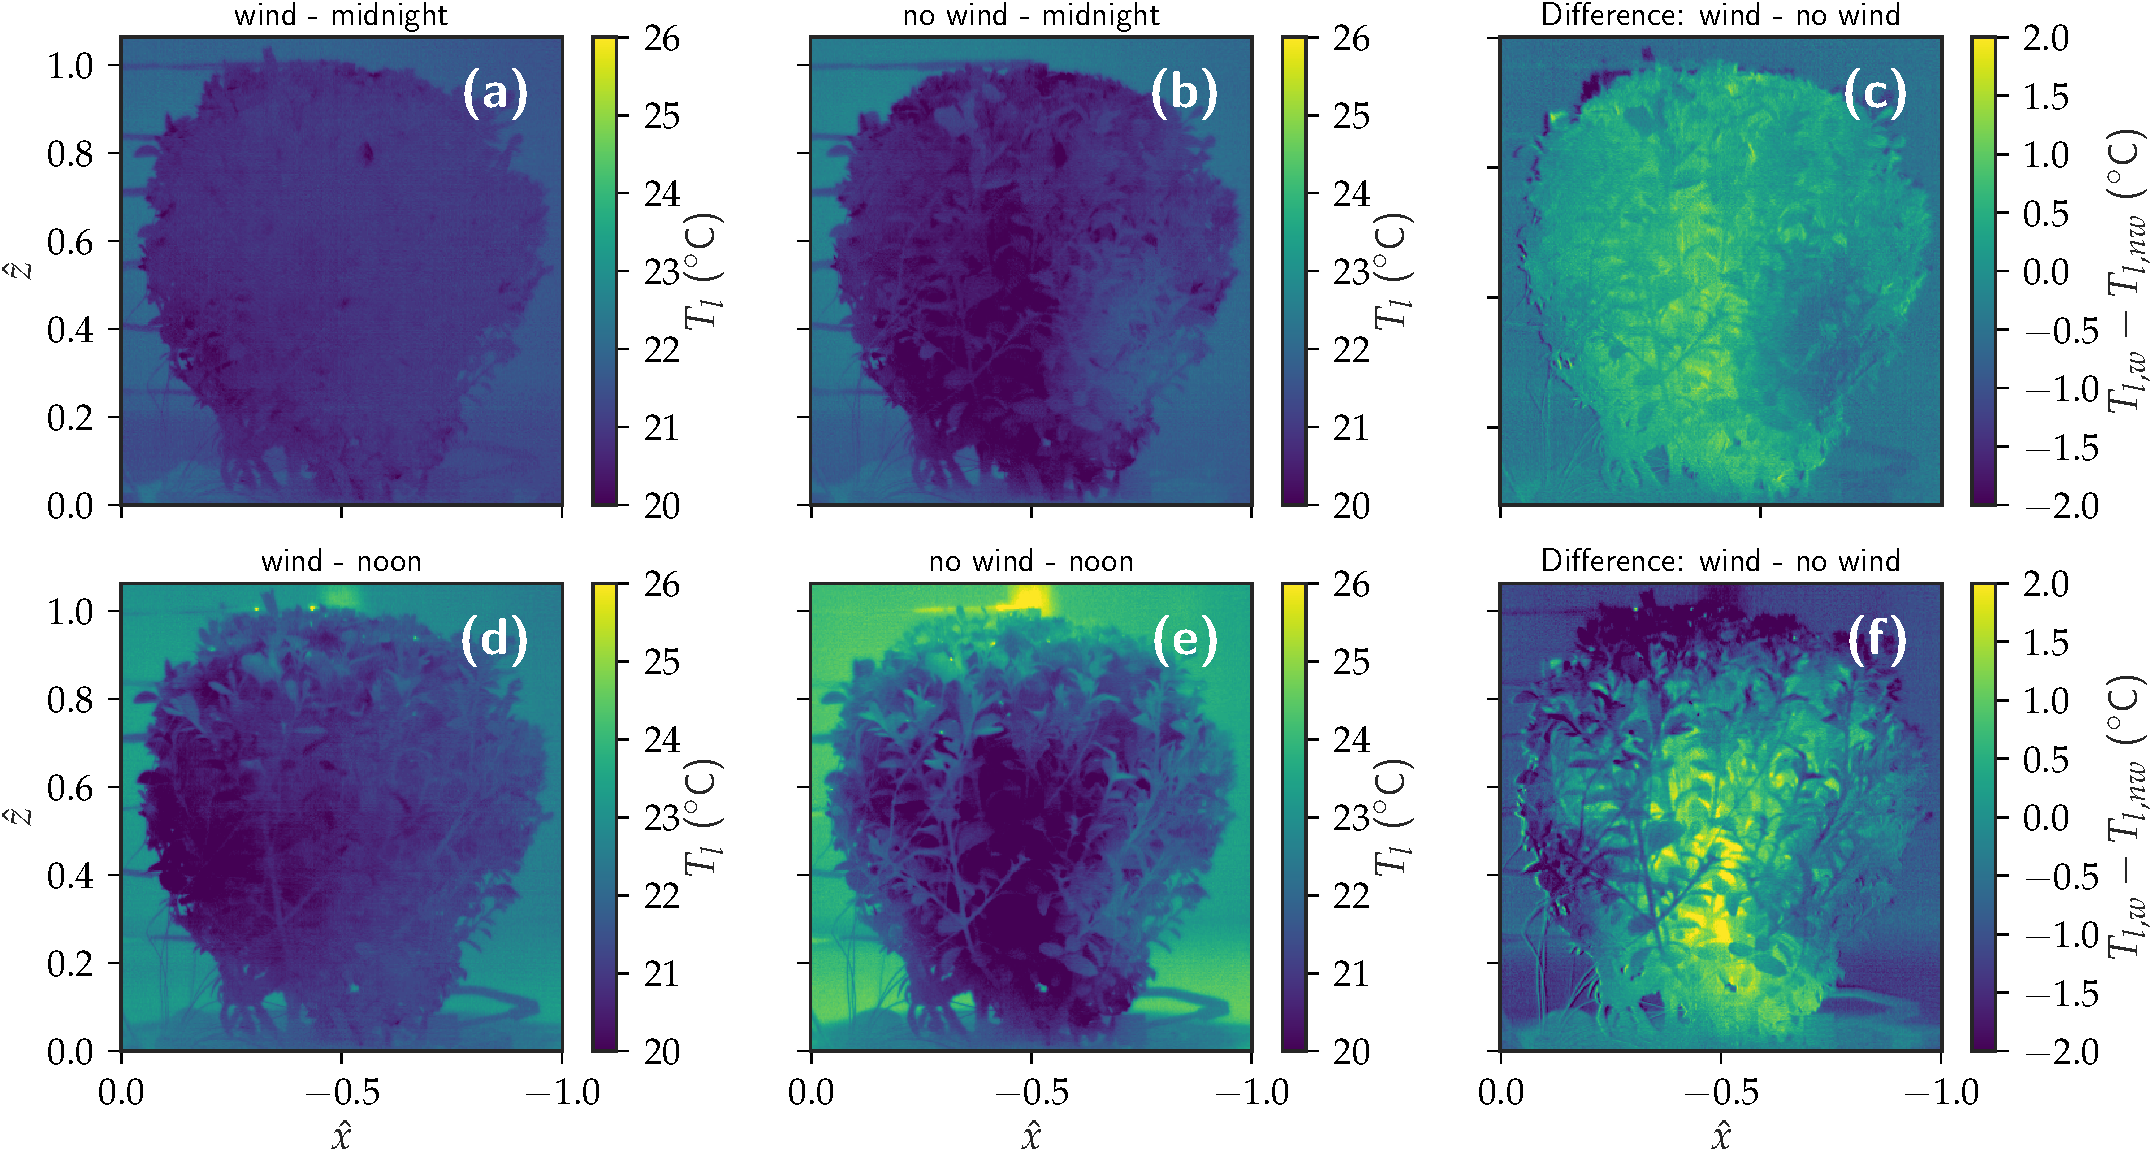
\includegraphics[width=\textwidth]{\figdir/IR_dayvsnight_windvsnowind_type2_v2-crop.pdf}
	\caption{Diurnal variation of leaf surface temperature $T_l$ ($^{\circ}$C) at \subfig{a}\subfig{b}\subfig{c} nighttime (midnight) (\subfig{d}\subfig{e}\subfig{f}  and midday (noon). The difference between \textit{wind} and \textit{no wind} condition is compared for \subfig{c} night and \subfig{f} day.}
	\label{fig:IR_dayvsnight_windvsnowind_type2_v2}
	\end{figure}


\subsection{Dynamic response of the plant}
\label{subsec:dynamic}

During the transition between day and night, a smaller time scale dynamic is observed, influenced by the abrupt changing in the environmental condition. \cref{fig:IRimage_phasediagram_type3} shows the spatiotemporal variability of streamwise-averaged leaf temperature $\langle T_l \rangle_x $ for \textit{no wind} and \textit{wind} condition. The figure shows the vertical variability in leaf temperature over the progression of the day. We see that, as observed with the internal microclimate of the plant (\cref{fig:figure_airtemperature_relativehumidity_profile}), the variability is only prevalent during the day time. Furthermore, the no wind condition shows stronger variability than the wind condition. During the day at no wind condition, a temperature spread from $19$ to $25$ $^{\circ}$C is observed. Moreover, we see that the leaf temperature is not only dependent on the vertical height, but also the time of the day. At the initial moments of dawn, the leaf temperatures quickly rise with highest temperatures observed at the plant canopy, showing a high gradient in leaf temperature where the leaves are exposed to solar radiation. We see that thereafter, the stomatal regulatory function takes over and a drastic decrease in foliage temperature is observable, especially in the middle regions of the foliage with  $T_l \approx 19$ $^{\circ}$C. As the day progress however, the cooling effect diminishes, and the foliage temperature starts to rise again. Just before dusk, a plant foliage temperature is similar to the onset of dawn, with high plant canopy temperatures. 

	\begin{figure}[t]
	\centering
	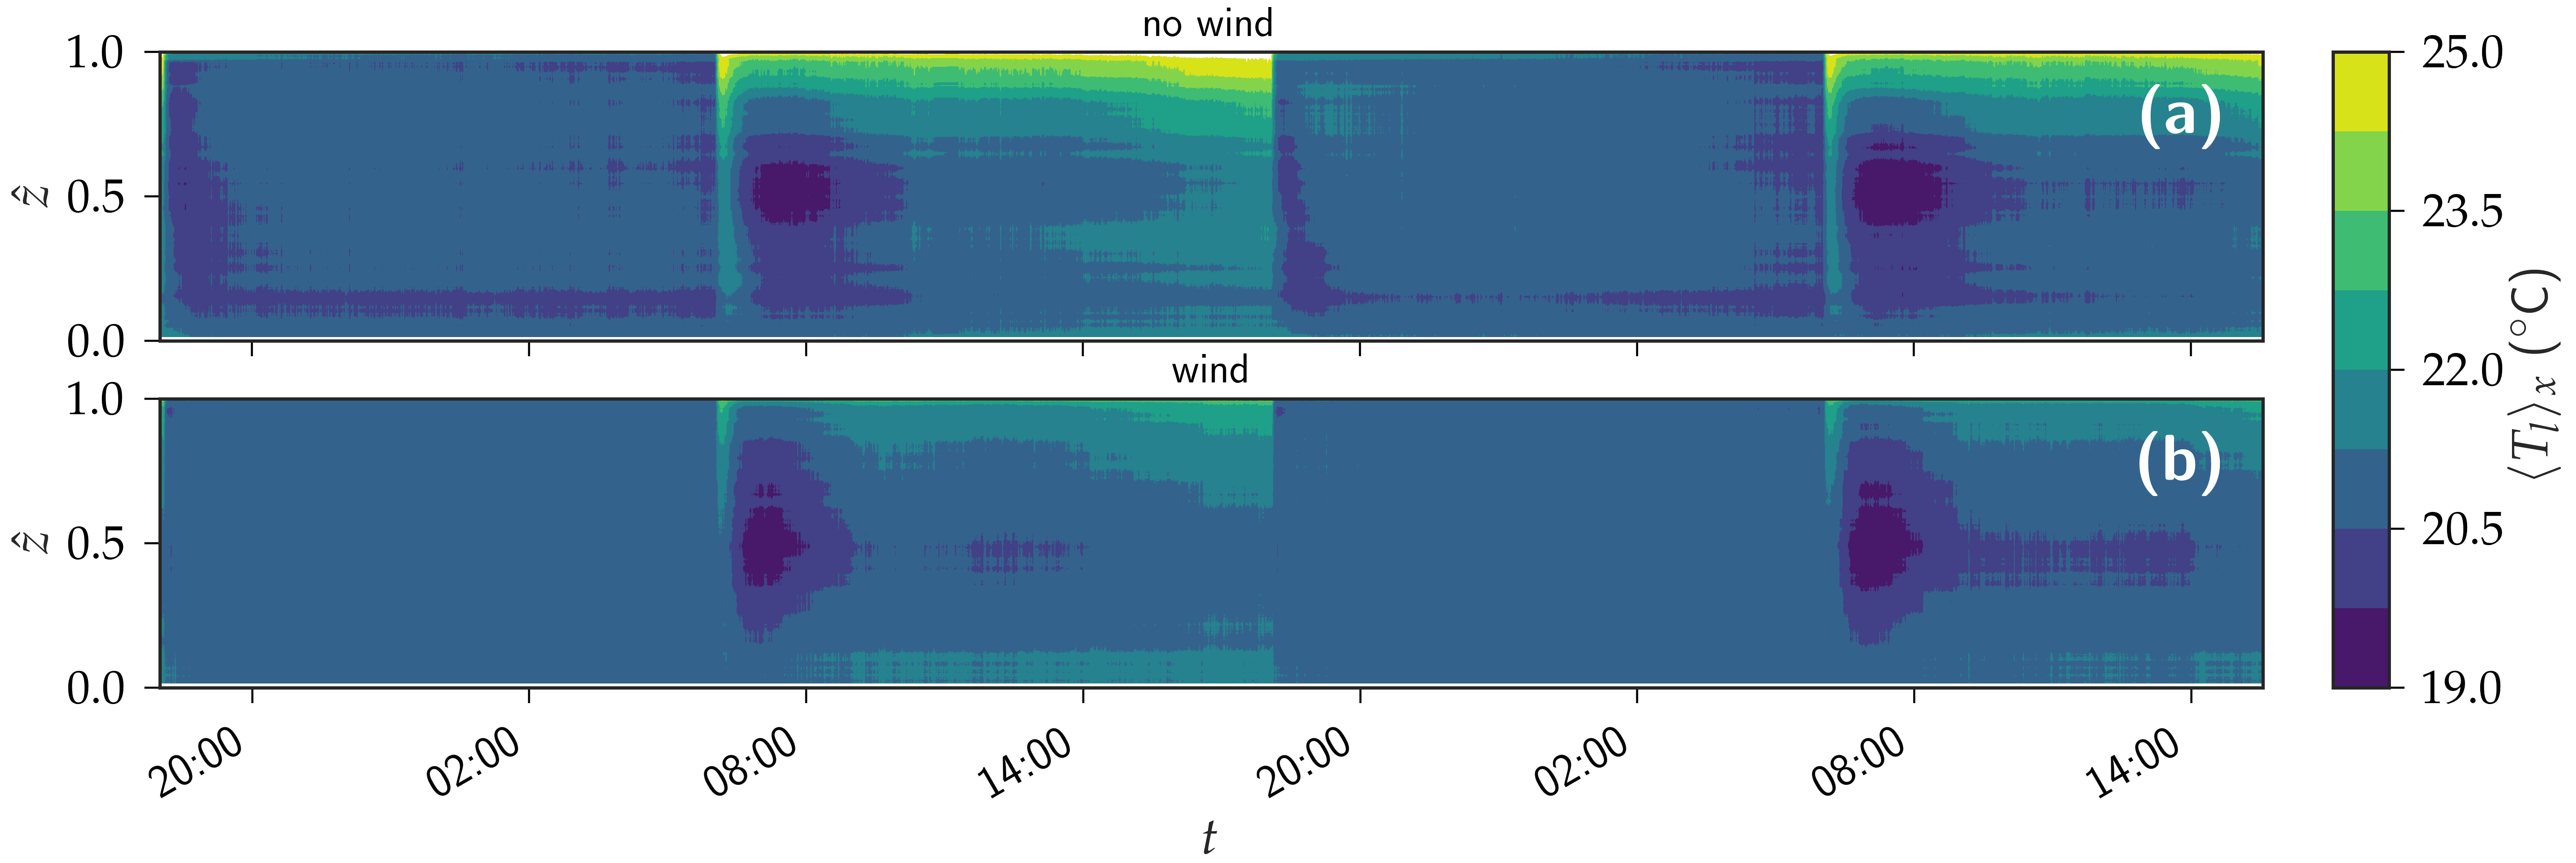
\includegraphics[width=\textwidth]{\figdir/IRimage_phasediagram_type3.png}
	\caption{Streamwise-averaged spatiotemporal variability of leaf temperature $\langle T_l \rangle_x$ ($^{\circ}$C) comparing \subfig{a} \textit{no wind} and \subfig{b} \textit{wind} condition.}
	\label{fig:IRimage_phasediagram_type3}
	\end{figure}

\cref{fig:Tprofile_2} shows the diurnal progress of the net spatial-averaged leaf temperature $\langle T_l \rangle_{xz}$ comparing wind and no wind condition. We notice that the no wind condition simply amplifies the characteristics that is present during the wind condition. Furthermore, we see that the day is composed of four unique stages: overshoot, overcorrection, equilibration and decay periods. The overshoot period is present at the initial stages of dawn where the leaves absorb solar radiation and stomata response has not been prevalent to provide the adequate transpiration rate. The delayed response of the plant results in the high overshoot of leaf temperature, which is compensated and corrected by the plant thereafter. However, we see that during the overcorrection period, the transpiration rate spikes, as evident from plant transpiration rate measurement, \cref{fig:figure_transpirationrate}, resulting in the drastic cooling measured. By midday, the stomatal response equilibrates the necessary transpiration rate and we observe a quasi-steady leaf temperature and transpiration rate (\cref{fig:figure_transpirationrate}) and in-foliage air temperature (\cref{fig:figure_airtemperature_humidity_v2}). Furthermore, it is shows that the equilibrium leaf temperature of plant foliage during no wind condition is higher than the wind condition. This is the result of the overall higher plant canopy temperature due to the reduces convective heat transfers. As the day progress, the leaf temperature transitions to the fourth stage with a slow increase in the leaf temperature. The observation correlates with the measured plant transpiration rate, \cref{fig:figure_transpirationrate}, where an equally decaying transpiration rate is observable. 

	\begin{figure}[t]
	\centering
	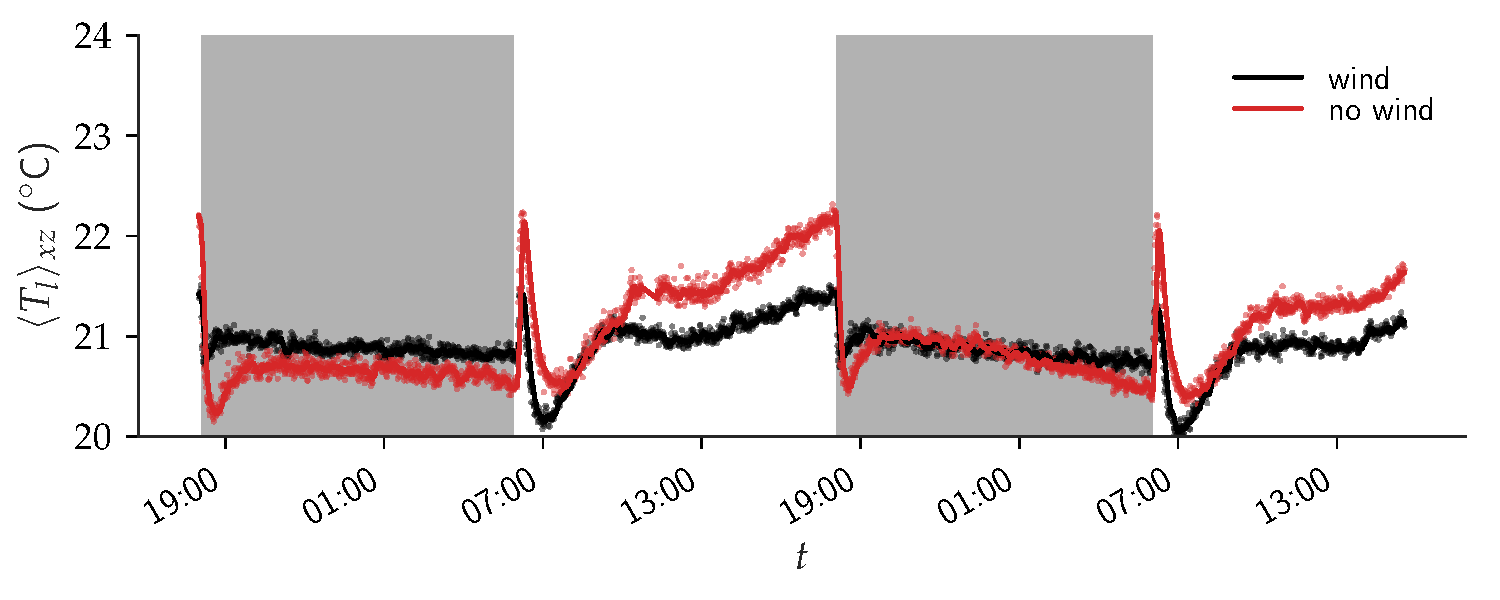
\includegraphics[width=\textwidth]{\figdir/Tprofile_2.pdf}
	\caption{Diurnal variation of spatially-averaged leaf temperature $\langle T_l \rangle$ ($^{\circ}$C) for \textit{wind} and \textit{no-wind} conditions.}
	\label{fig:Tprofile_2}
	\end{figure}

	\begin{figure}[t]
	\centering
	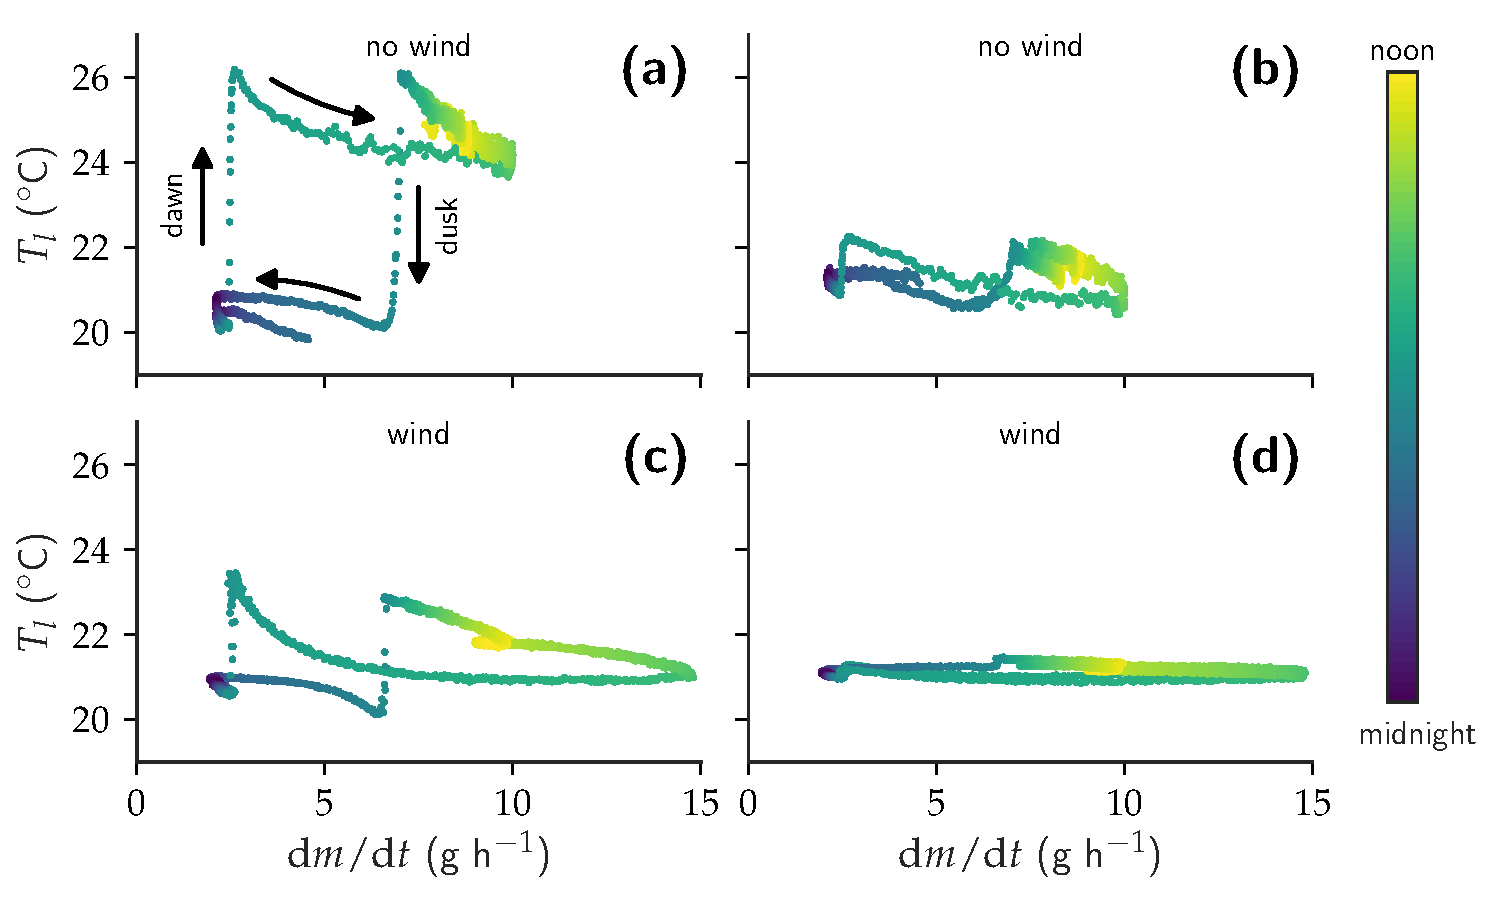
\includegraphics[width=\textwidth]{\figdir/hysteresis_transpirationrate_vs_temp_v2.pdf}
	\caption{Diurnal variation of $TR=\mathrm{d}m/\mathrm{d}t$ (g~h$^{-1}$) and leaf temperature for two wind conditions: \subfig{a}\subfig{b}  \textit{no-wind} and \subfig{c}\subfig{d}  with \textit{wind} ($U_{ref}=1$ m~s$^{-1}$). The leaf temperatures are obtained from \subfig{a}\subfig{c} plant canopy region and \subfig{b}\subfig{d}  near the ground region of the foliage.}
	\label{fig:hysteresis_transpirationrate_vs_temp_v2}
	\end{figure}

\cref{fig:hysteresis_transpirationrate_vs_temp_v2} shows a clearer hysteresis between net the leaf temperature and the net plant transpiration rate. The leaf temperatures of sunlight foliage and sunshade foliage are compared with the net plant transpiration. In all cases, a cyclic pattern of leaf temperature and transpiration rate is observable. Furthermore, we see that the hysteresis is amplified for the sunlight region during the no wind condition. At dawn, we see the overshoot as observed in \cref{fig:Tprofile_2}. After a delay, the stomata respond to the solar radiation and provide the necessary transpiration rate to cool the leaves. \cref{fig:IRimage_phasediagram_type3} shows this delayed cooling of the leaves observed through infrared thermography and the subsequent cooling of the air temperature, \cref{fig:figure_airtemperature_humidity_v2}, measured from the SHT sensors. However, towards dusk, we observe that the leaf temperatures slowly start to rice. An equivalent reduction in the plant transpiration rate is also observable from the hysteresis diagram, \cref{fig:hysteresis_transpirationrate_vs_temp_v2}. At the end of the photo-period, we observe a sudden drop in the leaf temperature. However, the plant transpiration rate is seen not to respond at the same rate as the decay in observed leaf temperature. Only after the leaf temperature equilibrated to a lower level is the stomata seen to respond, as indicated by the change in transpiration rate. The result is a cyclic nature of the plant transpiration rate, and the leaf temperature resulted from the delayed response of the plant. A similar observation of hysteresis between plant transpiration and the root water uptake has been known in the literature \citep{Dauzat2001, Williams1996}. An essential aspect of this hysteresis is that such dynamic response of the plant is difficult to parameterize in urban climate models of vegetation. Only after an explicit modeling on the water transport within the plant can such phenomena be captured \citep{Huang2017, Manzoni2011}.



\section{Conclusion}

The goal of the present study the response of the plant to the various environment, simultaneously measuring the plant morphology and the resulting flow condition. A high-resolution x-ray tomography approach is employed to measure various plant metrics such as porosity distribution, net plant leaf area and the leaf area density. Thereafter, the influence of heterogeneous foliage distribution on the internal plant microclimate and the wake flow turbulence is studied. The microclimate parameters such as air temperature and relative humidity are measured using SHT sensors, the net plant transpiration using a mass balance. Furthermore, an infrared thermography approach is employed to study the spatiotemporal variability in the leaf temperature due to multiple solar and wind conditions. To quantify the 3D wake flow time-averaged and turbulent kinetic energy, a stereoscopic particle image velocimetry (PIV) technique is employed to obtain multiple horizontal wake planes. The present study aims at answering the following questions: What are the spatial and temporal variability of the plant performance due to environmental conditions such as wind speed and solar radiation? What is the diurnal response of the plant? Therefore, the plant is subjected to two wind conditions: no wind and a wind tunnel set wind speed of $U_{ref}=1$ m~s$^{-1}$. Furthermore, at these two wind speeds, the plant is subjected to a solar cycle consisting of a 12-hour photoperiod with constant short-wave radiation at plant canopy of $100$ W~m$^{-2}$. A strong vertical variability in leaf temperature and the in-foliage air temperature was observed due to the solar radiation. At regions of high solar absorption, the leaf temperature and the air temperature are observed to be at highest. Whereas, further into the foliage, where most of the solar radiation is low, the transpiration provides noticeable cooling as observed through low air temperature and high relative humidity. At low wind conditions, the stagnated airflow inside the plant is seen to increase the measured cooling. 

Furthermore, the porosity variability due to the variability in plant morphology did not have a noticeable impact on the climate conditions. However, the wake turbulence characteristics as indicated by the turbulent kinetic energy, correlated with the variability in the porosity distribution. During the transition period of day and night, a hysteresis between net plant transpiration rate and the leaf temperature is observed. A sudden increase in leaf temperature resulted from the introduction of solar radiation resulted in a delayed response from the stomata as indicated by the net plant transpiration rate. This dynamic behavior usually presents in plant behavior is usually difficult to model, however, could have an influence when accurately modeling and quantifying the plant stress. Therefore, high-fidelity models of plant responses should take such dynamics that arise from water availability and the stomatal response delay into account, to accurately assess the impact of vegetation in a microclimate.


%\begin{figure}[t]
%\centering
%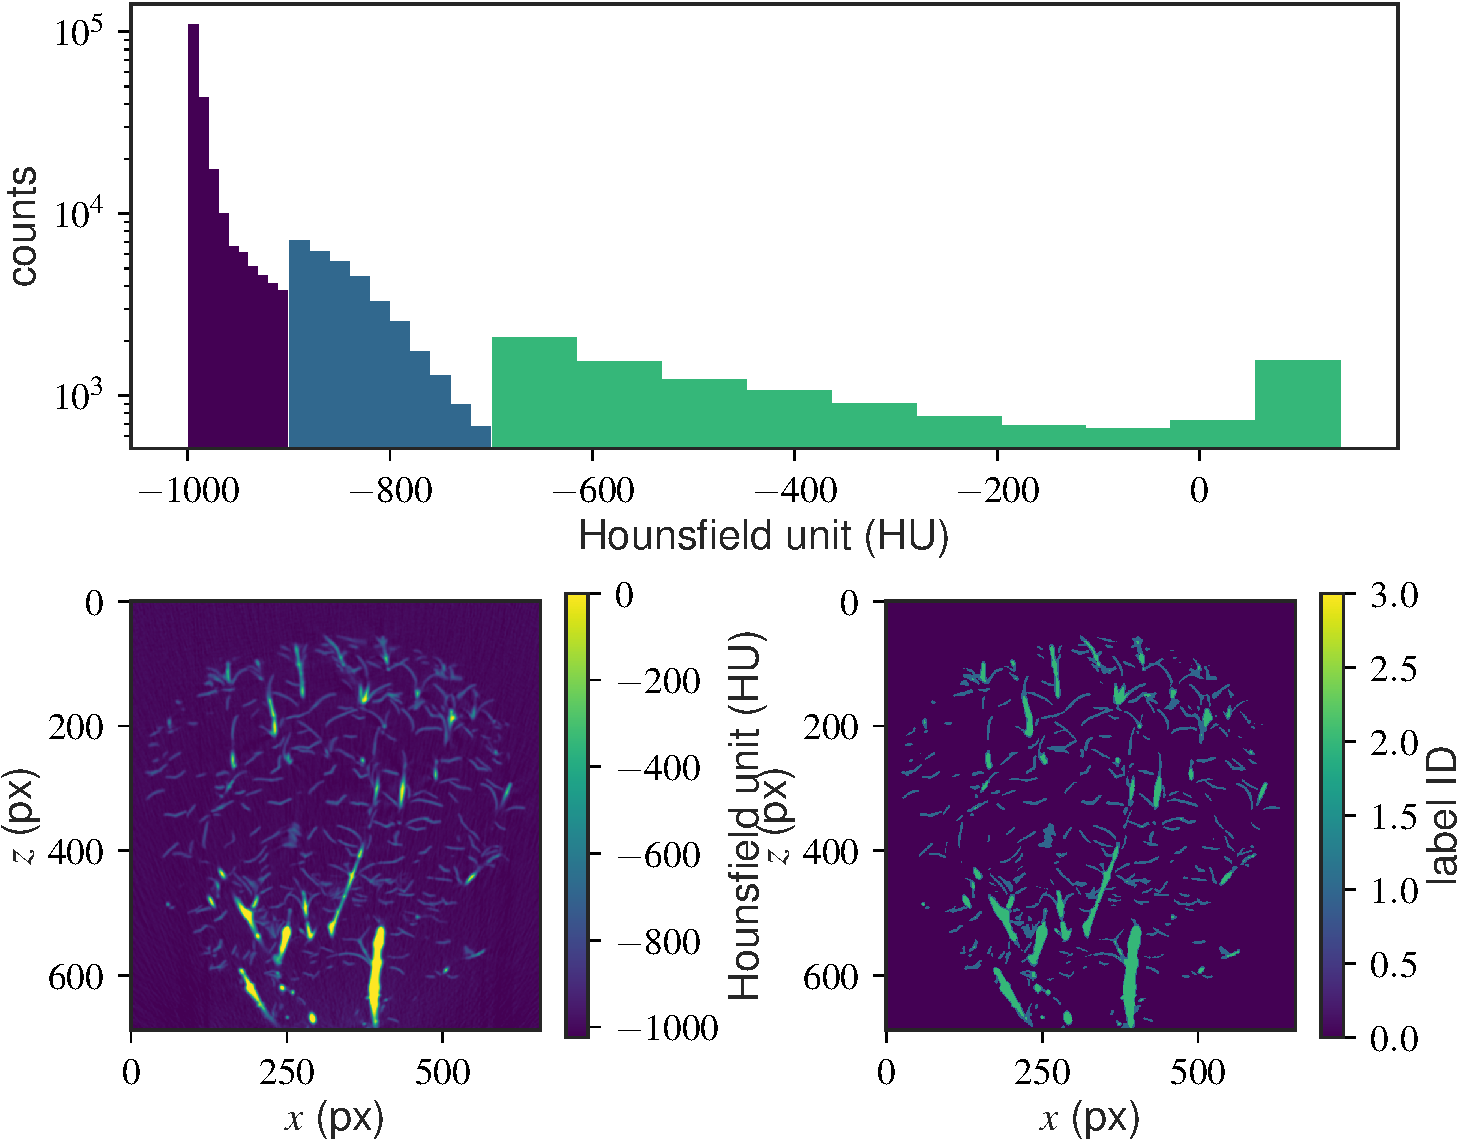
\includegraphics[width=\textwidth]{\figdir/figure_histogramsegentation-crop.pdf}
%\caption{Segmentation of the x-ray CT scan: a) original x-ray CT data, b) segmentation using user-defined histogram thresholding and c) segmentation using trainable WEKA segmentation and additional morphological operation (opening and closing). A sub-region of an image slice is shown for clarity.}
%\label{fig:figure_histogramsegentation}
%\end{figure}